\documentclass[aip,adv,preprint,floatfix]{revtex4-2}
\usepackage{amsmath,amssymb,bm}
\usepackage{tikz,pgfplots}
\usepgfplotslibrary{groupplots}
\pgfplotsset{compat=1.18}
\usepackage[hidelinks]{hyperref}
\begin{document}
\title{Phase Dynamics, Recurrence, and Relational Temporal Ordering in SEFI-DEFI-GWFM}
\author{Jason D. Dutton}
\email{sefidefi@outlook.com}
\affiliation{Independent Researcher, Castlewood, Virginia, USA}
\date{}
\begin{abstract}
We analyze operational temporal ordering in the Single Entity Field Interpretation (SEFI), Dynamic Entity Field Integration (DEFI), and Geometric Worldline Field Model (GWFM) through persistent oscillatory dynamics. The base identity action contains a harmonic Origin mode with conserved energy and advancing phase. Its cyclic phase has a unique continuous lift once dynamical orientation and an initial representative are specified. The lift orders occurrences, whereas the repeating state orbit admits no globally monotone instantaneous clock reading. Under specified assumptions, accumulated phase provides an operational temporal coordinate that supports relational descriptions of system evolution. We state the required phase observability, cycle record, positive phase speed, and solution uniqueness, and characterize when reconstructed observables are single-valued within one clock cycle. Exact full-state recurrence requires commensurate excited frequencies; bounded quasiperiodic structures can persist without exact finite reconstruction. Conditional frequency and lifted-phase locking supplies a shared calibrated reference without establishing attracting synchronization. An exact linear stability threshold, nonlinear confinement and equilibrium criteria, and a converged Floquet counterexample delimit persistent bounded evolution. Conservation, boundedness, recurrence, reconstruction, and clock recoverability are distinguished throughout. Standing waves are optional realizations rather than necessary assumptions. The results provide a conditional mechanism for operational temporal ordering, not elimination of the action's evolution parameter or a universal physical theory of time. We identify measurements and independent calibration needed to test a physical implementation.
\end{abstract}
\maketitle
\section{Introduction}
We examine how persistent oscillatory dynamics can supply an operational temporal coordinate within the proposed SEFI-DEFI-GWFM framework. The central result concerns accumulated phase: given directed dynamics, a nonzero phase-observable mode, and a continuing cycle record, it orders occurrences and parameterizes observable relations along a history. No spatial standing-wave assumption is needed. The construction describes temporal ordering operationally; it does not establish the fundamental absence of physical time.

The author's submitted manuscripts introduce worldline foundations \cite{r1}, scalar identity invariance \cite{r2}, unified stability surfaces \cite{r3}, displacement-engineered geometry \cite{r4}, photonic correction \cite{r5}, a coupled identity Lagrangian \cite{r6}, and a helical application \cite{r7}. They remain unpublished submitted works. The present paper is a self-contained analysis of a specified classical reduction, rather than independent validation of the companion interpretations.

The conservation law is for Origin energy, not for the value of phase. Phase progresses according to the dynamical equation. The phrase energy-conserving phase dynamics will mean phase evolution on an invariant nonzero-energy orbit. Conservation alone neither supplies a phase coordinate nor guarantees exact recurrence, boundedness of other coordinates, or recoverability of an observed state.

The distinction between cyclic state and ordered occurrence is central. A closed orbit has a cyclic phase coordinate, but the same instantaneous state repeats after each period. A phase lift and recorded cycles distinguish successive occurrences. Relational dynamics then follows from an invertible clock change along a selected history, with explicit requirements on phase speed and observable access.

Relational and periodic-clock descriptions are established topics \cite{r8}, \cite{r9}, \cite{r10}. The present classical construction neither inherits their quantum results nor makes operational cycle counting a gauge-invariant observable in a constrained theory. The new application is the combined consistency analysis of the specified identity coupling. Spectral, energy, Floquet, and phase-unwrapping methods are standard; the paper does not claim their discovery.

Sections 2–6 derive conservation, linear and nonlinear stability, and a driven counterexample. Section 7 separates exact reconstruction from persistent quasiperiodicity. Sections 8–12 connect the reduction to the submitted constructions, established physics, and reproducibility. Section 13 states phase-ordering, relational-observable, and shared-reference results with their limits. Section 14 sets out tests that would be needed for a physical implementation. The conclusion distinguishes operational temporal reconstruction from a universal theory of time.

\section{Model, conventions, and scope}
The scalar SEFI functional \cite{r2} combines Origin, Authorship, Sovereignty, and Warp contributions:

\begin{equation}
F=O(y)+A(y,\kappa)+S(y)+W(y).
\end{equation}
Invariance under an allowed transformation of $y$ is not automatically conservation along a dynamical solution. The component functions are unspecified. DEFI introduces a further modeling assumption: independent real coordinates $I=(I_O,I_A,I_S,I_W)$ with positive diagonal metric coefficients. We denote geometric curvature and torsion by $\kappa,\sigma$, avoiding confusion between torsion and the evolution parameter $\tau$.

\begin{equation}
M=\operatorname{diag}(\alpha,\beta,\gamma,\delta),\qquad \alpha,\beta,\gamma,\delta>0.
\end{equation}
The named coordinates are interpreted as upper-index components, with $I_a=M_{ab}I^b$. The DEFI kinetic expression \cite{r6} $M^{ab}\dot I_a\dot I_b$ then equals $M_{ab}\dot I^a\dot I^b$, consistently with its displayed identity equations. Dots denote derivatives with respect to dimensionless $\tau$. We adopt the source common unit oscillator frequency; no physical calibration of the frequency or identity coordinates is supplied.

\begin{equation}
L_I=\frac12\dot I^T M\dot I-\frac12I^TMI-U,
\end{equation}
\begin{equation}
U=\mu_1(I_A)\kappa^2I_S+\mu_2(I_A)\sigma^2I_W.
\end{equation}
We prescribe $\kappa,\sigma$ in the identity equations. Constant geometry gives an autonomous identity reduction; periodically prescribed geometry gives a driven reduction. Neither is a solution of the full spacetime variational problem. Coupling functions are real $C^2$, and $C^3$ when using nonlinear Taylor expansions. Variation gives

\begin{equation}
\ddot I_O+I_O=0,
\end{equation}
\begin{equation}
\beta\ddot I_A+\beta I_A+\mu_1^\prime(I_A)\kappa^2I_S+\mu_2^\prime(I_A)\sigma^2I_W=0,
\end{equation}
\begin{equation}
\gamma\ddot I_S+\gamma I_S+\mu_1(I_A)\kappa^2=0,
\end{equation}
\begin{equation}
\delta\ddot I_W+\delta I_W+\mu_2(I_A)\sigma^2=0.
\end{equation}
No empirical meaning is assigned to the coordinate names merely by writing these equations. In particular, a coordinate-sector energy is not identified with physical particle identity.

\section{Origin energy and cyclic phase}
Proposition 1. For every prescribed geometry history and solution of the other identity equations, the following Origin energy is nonnegative and conserved:

\begin{equation}
Q_O=\frac{\alpha}{2}(\dot I_O^2+I_O^2).
\end{equation}
Proof. Differentiation gives $\dot Q_O=\alpha\dot I_O(\ddot I_O+I_O)=0$. For nonzero amplitude,

\begin{equation}
I_O=A\cos(\tau+\theta_0),\quad \dot I_O=-A\sin(\tau+\theta_0),\quad Q_O=\frac{\alpha A^2}{2}.
\end{equation}
The pair $(I_O,-\dot I_O)$ defines $\theta_O=\tau+\theta_0$ modulo $2\pi$. Both quadratures, or an equivalent history prescription, are needed to infer phase; $I_O$ alone is ambiguous. At $Q_O=0$ the solution vanishes and oscillator phase is undefined.

Origin is decoupled in the stated action. Its energy can remain constant while other coordinates grow, drift, or fail to recur. Different states and phases share the same $Q_O$, so it is not a complete state identifier. This is subsystem conservation, not a global stability theorem.

The conservation statement agrees with the subsystem time-translation energy relation underlying Noether's theorem \cite{r11}. It is not a separate demonstration that the scalar SEFI functional is a Noether charge. The identity coordinates and the conserved energy remain distinct mathematical objects.

\section{Linear coupling at constant geometry}
Set $\kappa=\kappa_0$, $\sigma=\sigma_0$ and choose $\mu_1(I_A)=g_1I_A$, $\mu_2(I_A)=g_2I_A$. These are explicit allowed functions, not fits to observations. Define

\begin{equation}
X=(\sqrt{\beta}I_A,\sqrt{\gamma}I_S,\sqrt{\delta}I_W)^T,
\end{equation}
\begin{equation}
a=\frac{g_1\kappa_0^2}{\sqrt{\beta\gamma}},\quad b=\frac{g_2\sigma_0^2}{\sqrt{\beta\delta}},\quad r=\sqrt{a^2+b^2}.
\end{equation}
The equation is $\ddot X+BX=0$, with the symmetric matrix specified by

\begin{equation}
B=\begin{pmatrix}1&a&b\\a&1&0\\b&0&1\end{pmatrix}.
\end{equation}
Proposition 2. The stiffness eigenvalues are $1-r$, $1$, and $1+r$. For $r>0$ an orthonormal eigenbasis is

\begin{equation}
e_\pm=\frac1{\sqrt2}(1,\pm a/r,\pm b/r)^T,\quad e_0=(0,-b/r,a/r)^T.
\end{equation}
Proof. The direction $(a,b)/r$ in the Sovereignty-Warp plane couples to Authorship with strength $r$. Its orthogonal complement has eigenvalue one. The remaining two-coordinate block has diagonal entries one and off-diagonal entries $r$, giving eigenvalues $1\pm r$. At $r=0$, $B$ is the identity matrix. Figure 1 shows the spectrum.

\begin{figure}[htbp]\centering
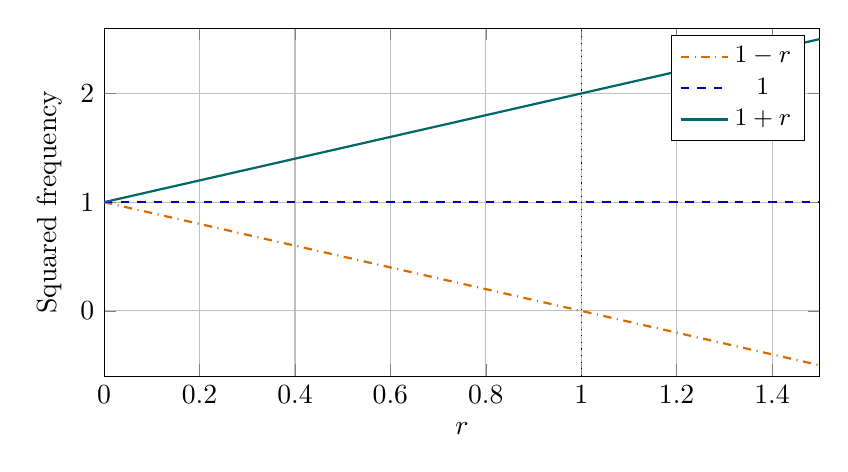
\begin{tikzpicture}
\begin{axis}[width=.88\textwidth,height=6cm,grid=major,legend style={font=\small},xlabel={$r$},ylabel={Squared frequency},ymin=-.6,ymax=2.6,xmin=0,xmax=1.5]
\addplot[orange!85!black,dashdotted,thick] coordinates{(0,1) (0.015,0.985) (0.03,0.97) (0.045,0.955) (0.06,0.94) (0.075,0.925) (0.09,0.91) (0.105,0.895) (0.12,0.88) (0.135,0.865) (0.15,0.85) (0.165,0.835) (0.18,0.82) (0.195,0.805) (0.21,0.79) (0.225,0.775) (0.24,0.76) (0.255,0.745) (0.27,0.73) (0.285,0.715) (0.3,0.7) (0.315,0.685) (0.33,0.67) (0.345,0.655) (0.36,0.64) (0.375,0.625) (0.39,0.61) (0.405,0.595) (0.42,0.58) (0.435,0.565) (0.45,0.55) (0.465,0.535) (0.48,0.52) (0.495,0.505) (0.51,0.49) (0.525,0.475) (0.54,0.46) (0.555,0.445) (0.57,0.43) (0.585,0.415) (0.6,0.4) (0.615,0.385) (0.63,0.37) (0.645,0.355) (0.66,0.34) (0.675,0.325) (0.69,0.31) (0.705,0.295) (0.72,0.28) (0.735,0.265) (0.75,0.25) (0.765,0.235) (0.78,0.22) (0.795,0.205) (0.81,0.19) (0.825,0.175) (0.84,0.16) (0.855,0.145) (0.87,0.13) (0.885,0.115) (0.9,0.1) (0.915,0.085) (0.93,0.07) (0.945,0.055) (0.96,0.04) (0.975,0.025) (0.99,0.01) (1.005,-0.005) (1.02,-0.02) (1.035,-0.035) (1.05,-0.05) (1.065,-0.065) (1.08,-0.08) (1.095,-0.095) (1.11,-0.11) (1.125,-0.125) (1.14,-0.14) (1.155,-0.155) (1.17,-0.17) (1.185,-0.185) (1.2,-0.2) (1.215,-0.215) (1.23,-0.23) (1.245,-0.245) (1.26,-0.26) (1.275,-0.275) (1.29,-0.29) (1.305,-0.305) (1.32,-0.32) (1.335,-0.335) (1.35,-0.35) (1.365,-0.365) (1.38,-0.38) (1.395,-0.395) (1.41,-0.41) (1.425,-0.425) (1.44,-0.44) (1.455,-0.455) (1.47,-0.47) (1.485,-0.485) (1.5,-0.5)};
\addlegendentry{$1-r$}
\addplot[blue!70!black,dashed,thick] coordinates{(0,1) (0.015,1) (0.03,1) (0.045,1) (0.06,1) (0.075,1) (0.09,1) (0.105,1) (0.12,1) (0.135,1) (0.15,1) (0.165,1) (0.18,1) (0.195,1) (0.21,1) (0.225,1) (0.24,1) (0.255,1) (0.27,1) (0.285,1) (0.3,1) (0.315,1) (0.33,1) (0.345,1) (0.36,1) (0.375,1) (0.39,1) (0.405,1) (0.42,1) (0.435,1) (0.45,1) (0.465,1) (0.48,1) (0.495,1) (0.51,1) (0.525,1) (0.54,1) (0.555,1) (0.57,1) (0.585,1) (0.6,1) (0.615,1) (0.63,1) (0.645,1) (0.66,1) (0.675,1) (0.69,1) (0.705,1) (0.72,1) (0.735,1) (0.75,1) (0.765,1) (0.78,1) (0.795,1) (0.81,1) (0.825,1) (0.84,1) (0.855,1) (0.87,1) (0.885,1) (0.9,1) (0.915,1) (0.93,1) (0.945,1) (0.96,1) (0.975,1) (0.99,1) (1.005,1) (1.02,1) (1.035,1) (1.05,1) (1.065,1) (1.08,1) (1.095,1) (1.11,1) (1.125,1) (1.14,1) (1.155,1) (1.17,1) (1.185,1) (1.2,1) (1.215,1) (1.23,1) (1.245,1) (1.26,1) (1.275,1) (1.29,1) (1.305,1) (1.32,1) (1.335,1) (1.35,1) (1.365,1) (1.38,1) (1.395,1) (1.41,1) (1.425,1) (1.44,1) (1.455,1) (1.47,1) (1.485,1) (1.5,1)};
\addlegendentry{$1$}
\addplot[teal!80!black,thick] coordinates{(0,1) (0.015,1.015) (0.03,1.03) (0.045,1.045) (0.06,1.06) (0.075,1.075) (0.09,1.09) (0.105,1.105) (0.12,1.12) (0.135,1.135) (0.15,1.15) (0.165,1.165) (0.18,1.18) (0.195,1.195) (0.21,1.21) (0.225,1.225) (0.24,1.24) (0.255,1.255) (0.27,1.27) (0.285,1.285) (0.3,1.3) (0.315,1.315) (0.33,1.33) (0.345,1.345) (0.36,1.36) (0.375,1.375) (0.39,1.39) (0.405,1.405) (0.42,1.42) (0.435,1.435) (0.45,1.45) (0.465,1.465) (0.48,1.48) (0.495,1.495) (0.51,1.51) (0.525,1.525) (0.54,1.54) (0.555,1.555) (0.57,1.57) (0.585,1.585) (0.6,1.6) (0.615,1.615) (0.63,1.63) (0.645,1.645) (0.66,1.66) (0.675,1.675) (0.69,1.69) (0.705,1.705) (0.72,1.72) (0.735,1.735) (0.75,1.75) (0.765,1.765) (0.78,1.78) (0.795,1.795) (0.81,1.81) (0.825,1.825) (0.84,1.84) (0.855,1.855) (0.87,1.87) (0.885,1.885) (0.9,1.9) (0.915,1.915) (0.93,1.93) (0.945,1.945) (0.96,1.96) (0.975,1.975) (0.99,1.99) (1.005,2.005) (1.02,2.02) (1.035,2.035) (1.05,2.05) (1.065,2.065) (1.08,2.08) (1.095,2.095) (1.11,2.11) (1.125,2.125) (1.14,2.14) (1.155,2.155) (1.17,2.17) (1.185,2.185) (1.2,2.2) (1.215,2.215) (1.23,2.23) (1.245,2.245) (1.26,2.26) (1.275,2.275) (1.29,2.29) (1.305,2.305) (1.32,2.32) (1.335,2.335) (1.35,2.35) (1.365,2.365) (1.38,2.38) (1.395,2.395) (1.41,2.41) (1.425,2.425) (1.44,2.44) (1.455,2.455) (1.47,2.47) (1.485,2.485) (1.5,2.5)};
\addlegendentry{$1+r$}
\addplot[black,dotted] coordinates{(1,-0.6) (1,2.6)};
\end{axis}
\end{tikzpicture}
\caption{Squared normal-mode frequencies of the constant-geometry linear reduction. The lower branch reaches zero at $r=1$ and becomes negative above it. These are exact model eigenvalues, not measured spectra.}
\end{figure}
Proposition 3. Every linear identity solution is bounded in coordinates and velocities for $0\leq r<1$. At $r=1$, zero-mode velocity can produce secular drift. For $r>1$, exponentially growing solutions exist.

Proof. The reduced energy is conserved:

\begin{equation}
H_R=\frac12(|\dot X|^2+X^TBX),\quad \dot H_R=0.
\end{equation}
Below threshold positive definiteness gives

\begin{equation}
H_R\geq\frac12|\dot X|^2+\frac12(1-r)|X|^2.
\end{equation}
At $r=1$ the soft coordinate obeys $\ddot\eta_-=0$, hence $\eta_-=C+D\tau$. Above threshold it obeys $\ddot\eta_--(r-1)\eta_-=0$, admitting $\exp(\sqrt{r-1}\tau)$ growth. Special initial conditions can suppress the growing component, but its existence makes the equilibrium unstable.

The first-order zero-mode block at threshold is not diagonalizable; eigenvalues with nonpositive real parts alone would miss drift. Positive stiffness gives Lyapunov stability, not attraction. Conservative harmonic motion does not relax to equilibrium. Figure 2 compares the behaviors with identical Origin energy.

\begin{figure}[htbp]\centering
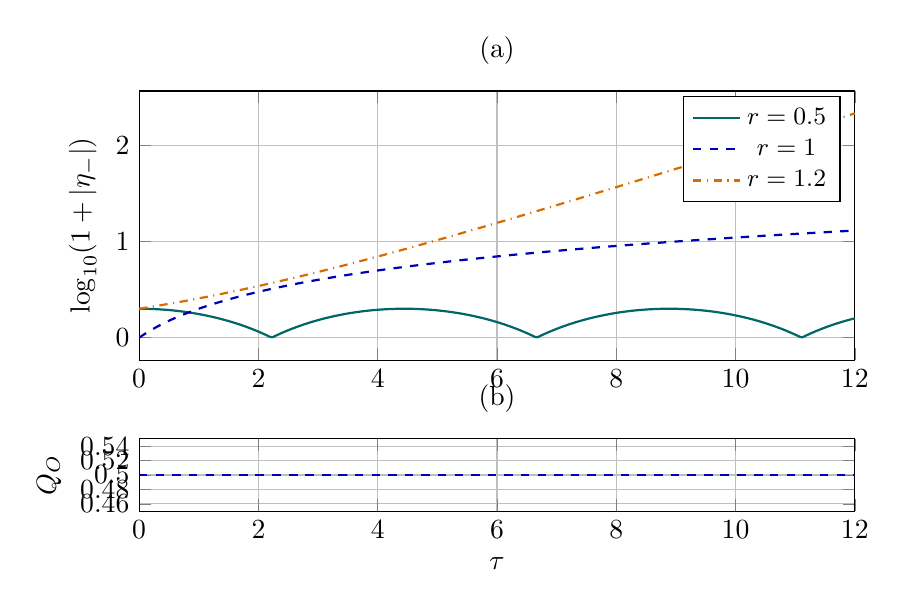
\begin{tikzpicture}
\begin{groupplot}[group style={group size=1 by 2,vertical sep=1cm},width=.88\textwidth,height=5cm,grid=major,xmin=0,xmax=12]
\nextgroupplot[ylabel={$\log_{10}(1+|\eta_-|)$},title={(a)},legend style={font=\small}]
\addplot[teal!80!black,thick] coordinates{(0,0.30103) (0.04,0.30094313) (0.08,0.30068251) (0.12,0.30024803) (0.16,0.29963951) (0.2,0.29885671) (0.24,0.29789932) (0.28,0.29676694) (0.32,0.29545913) (0.36,0.29397535) (0.4,0.292315) (0.44,0.2904774) (0.48,0.28846181) (0.52,0.2862674) (0.56,0.28389325) (0.6,0.28133839) (0.64,0.27860174) (0.68,0.27568216) (0.72,0.27257842) (0.76,0.26928919) (0.8,0.26581306) (0.84,0.26214853) (0.88,0.25829401) (0.92,0.2542478) (0.96,0.2500081) (1,0.24557302) (1.04,0.24094055) (1.08,0.23610858) (1.12,0.23107487) (1.16,0.22583706) (1.2,0.2203927) (1.24,0.21473916) (1.28,0.2088737) (1.32,0.20279345) (1.36,0.19649538) (1.4,0.1899763) (1.44,0.18323287) (1.48,0.17626157) (1.52,0.16905873) (1.56,0.16162047) (1.6,0.15394272) (1.64,0.14602121) (1.68,0.13785146) (1.72,0.12942874) (1.76,0.1207481) (1.8,0.11180433) (1.84,0.10259197) (1.88,0.09310524) (1.92,0.083338093) (1.96,0.073284145) (2,0.06293668) (2.04,0.052288619) (2.08,0.041332499) (2.12,0.030060448) (2.16,0.018464157) (2.2,0.006534851) (2.24,0.0056619547) (2.28,0.017615615) (2.32,0.029235607) (2.36,0.040530744) (2.4,0.051509366) (2.44,0.062179377) (2.48,0.072548265) (2.52,0.082623139) (2.56,0.092410739) (2.6,0.10191747) (2.64,0.11114941) (2.68,0.12011235) (2.72,0.12881178) (2.76,0.13725292) (2.8,0.14544075) (2.84,0.15338) (2.88,0.16107517) (2.92,0.16853055) (2.96,0.17575023) (3,0.18273808) (3.04,0.18949782) (3.08,0.19603295) (3.12,0.20234685) (3.16,0.20844269) (3.2,0.21432353) (3.24,0.21999225) (3.28,0.22545161) (3.32,0.23070421) (3.36,0.23575255) (3.4,0.24059899) (3.44,0.24524577) (3.48,0.24969501) (3.52,0.25394872) (3.56,0.25800882) (3.6,0.2618771) (3.64,0.26555526) (3.68,0.26904492) (3.72,0.27234757) (3.76,0.27546464) (3.8,0.27839745) (3.84,0.28114724) (3.88,0.28371517) (3.92,0.2861023) (3.96,0.28830964) (4,0.29033809) (4.04,0.29218849) (4.08,0.29386159) (4.12,0.29535808) (4.16,0.29667855) (4.2,0.29782356) (4.24,0.29879355) (4.28,0.29958892) (4.32,0.30021) (4.36,0.30065701) (4.4,0.30093016) (4.44,0.30102954) (4.48,0.3009552) (4.52,0.30070711) (4.56,0.30028516) (4.6,0.29968919) (4.64,0.29891896) (4.68,0.29797416) (4.72,0.29685441) (4.76,0.29555926) (4.8,0.29408818) (4.84,0.29244058) (4.88,0.29061579) (4.92,0.28861305) (4.96,0.28643155) (5,0.28407039) (5.04,0.28152859) (5.08,0.27880508) (5.12,0.27589873) (5.16,0.2728083) (5.2,0.26953249) (5.24,0.26606988) (5.28,0.26241898) (5.32,0.25857821) (5.36,0.25454587) (5.4,0.25032018) (5.44,0.24589925) (5.48,0.24128107) (5.52,0.23646355) (5.56,0.23144446) (5.6,0.22622145) (5.64,0.22079205) (5.68,0.21515368) (5.72,0.20930359) (5.76,0.20323892) (5.8,0.19695665) (5.84,0.19045361) (5.88,0.18372646) (5.92,0.17677172) (5.96,0.16958569) (6,0.16216453) (6.04,0.15450419) (6.08,0.14660039) (6.12,0.13844868) (6.16,0.13004435) (6.2,0.12138248) (6.24,0.11245785) (6.28,0.10326504) (6.32,0.093798284) (6.36,0.084051557) (6.4,0.074018501) (6.44,0.063692423) (6.48,0.053066271) (6.52,0.042132612) (6.56,0.030883604) (6.6,0.01931097) (6.64,0.0074059695) (6.68,0.004787277) (6.72,0.016765339) (6.76,0.02840908) (6.8,0.039727346) (6.84,0.050728511) (6.88,0.061420509) (6.92,0.071810858) (6.96,0.081906692) (7,0.09171478) (7.04,0.10124155) (7.08,0.1104931) (7.12,0.11947524) (7.16,0.12819348) (7.2,0.13665306) (7.24,0.14485899) (7.28,0.152816) (7.32,0.16052862) (7.36,0.16800115) (7.4,0.17523768) (7.44,0.18224212) (7.48,0.18901817) (7.52,0.19556938) (7.56,0.20189911) (7.6,0.20801057) (7.64,0.21390681) (7.68,0.21959072) (7.72,0.22506508) (7.76,0.2303325) (7.8,0.23539548) (7.84,0.24025639) (7.88,0.24491749) (7.92,0.24938089) (7.96,0.25364864) (8,0.25772263) (8.04,0.26160467) (8.08,0.26529649) (8.12,0.26879968) (8.16,0.27211576) (8.2,0.27524616) (8.24,0.2781922) (8.28,0.28095515) (8.32,0.28353615) (8.36,0.28593628) (8.4,0.28815655) (8.44,0.29019786) (8.48,0.29206106) (8.52,0.29374692) (8.56,0.29525611) (8.6,0.29658926) (8.64,0.29774689) (8.68,0.29872948) (8.72,0.29953743) (8.76,0.30017106) (8.8,0.30063061) (8.84,0.30091629) (8.88,0.30102819) (8.92,0.30096637) (8.96,0.3007308) (9,0.30032139) (9.04,0.29973797) (9.08,0.29898031) (9.12,0.29804811) (9.16,0.29694098) (9.2,0.29565848) (9.24,0.29420011) (9.28,0.29256525) (9.32,0.29075325) (9.36,0.28876336) (9.4,0.28659478) (9.44,0.2842466) (9.48,0.28171785) (9.52,0.27900748) (9.56,0.27611434) (9.6,0.27303722) (9.64,0.26977482) (9.68,0.26632572) (9.72,0.26268844) (9.76,0.25886141) (9.8,0.25484294) (9.84,0.25063125) (9.88,0.24622445) (9.92,0.24162056) (9.96,0.23681748) (10,0.23181299) (10.04,0.22660476) (10.08,0.22119033) (10.12,0.2155671) (10.16,0.20973237) (10.2,0.20368326) (10.24,0.19741678) (10.28,0.19092976) (10.32,0.18421888) (10.36,0.17728066) (10.4,0.17011143) (10.44,0.16270735) (10.48,0.15506438) (10.52,0.14717828) (10.56,0.13904459) (10.6,0.13065863) (10.64,0.12201549) (10.68,0.11310998) (10.72,0.10393669) (10.76,0.094489874) (10.8,0.084763534) (10.84,0.074751334) (10.88,0.064446607) (10.92,0.053842327) (10.96,0.042931088) (11,0.031705079) (11.04,0.020156057) (11.08,0.0082753137) (11.12,0.0039108143) (11.16,0.015913327) (11.2,0.027580862) (11.24,0.0389223) (11.28,0.04994605) (11.32,0.060660074) (11.36,0.071071921) (11.4,0.081188752) (11.44,0.091017359) (11.48,0.10056419) (11.52,0.10983538) (11.56,0.11883675) (11.6,0.12757383) (11.64,0.13605189) (11.68,0.14427594) (11.72,0.15225074) (11.76,0.15998082) (11.8,0.16747052) (11.84,0.17472392) (11.88,0.18174496) (11.92,0.18853736) (11.96,0.19510466) (12,0.20145024)};
\addlegendentry{$r=0.5$}
\addplot[blue!70!black,dashed,thick] coordinates{(0,0) (0.04,0.017033339) (0.08,0.033423755) (0.12,0.049218023) (0.16,0.064457989) (0.2,0.079181246) (0.24,0.093421685) (0.28,0.10720997) (0.32,0.12057393) (0.36,0.13353891) (0.4,0.14612804) (0.44,0.15836249) (0.48,0.17026172) (0.52,0.18184359) (0.56,0.1931246) (0.6,0.20411998) (0.64,0.21484385) (0.68,0.22530928) (0.72,0.23552845) (0.76,0.24551267) (0.8,0.25527251) (0.84,0.26481782) (0.88,0.27415785) (0.92,0.28330123) (0.96,0.29225607) (1,0.30103) (1.04,0.30963017) (1.08,0.31806333) (1.12,0.32633586) (1.16,0.33445375) (1.2,0.34242268) (1.24,0.35024802) (1.28,0.35793485) (1.32,0.36548798) (1.36,0.372912) (1.4,0.38021124) (1.44,0.38738983) (1.48,0.39445168) (1.52,0.40140054) (1.56,0.40823997) (1.6,0.41497335) (1.64,0.42160393) (1.68,0.42813479) (1.72,0.4345689) (1.76,0.44090908) (1.8,0.44715803) (1.84,0.45331834) (1.88,0.45939249) (1.92,0.46538285) (1.96,0.47129171) (2,0.47712125) (2.04,0.48287358) (2.08,0.48855072) (2.12,0.49415459) (2.16,0.49968708) (2.2,0.50514998) (2.24,0.51054501) (2.28,0.51587384) (2.32,0.52113808) (2.36,0.52633928) (2.4,0.53147892) (2.44,0.53655844) (2.48,0.54157924) (2.52,0.54654266) (2.56,0.55145) (2.6,0.5563025) (2.64,0.56110138) (2.68,0.56584782) (2.72,0.57054294) (2.76,0.57518784) (2.8,0.5797836) (2.84,0.58433122) (2.88,0.58883173) (2.92,0.59328607) (2.96,0.59769519) (3,0.60205999) (3.04,0.60638137) (3.08,0.61066016) (3.12,0.61489722) (3.16,0.61909333) (3.2,0.62324929) (3.24,0.62736586) (3.28,0.63144377) (3.32,0.63548375) (3.36,0.63948649) (3.4,0.64345268) (3.44,0.64738297) (3.48,0.65127801) (3.52,0.65513843) (3.56,0.65896484) (3.6,0.66275783) (3.64,0.66651798) (3.68,0.67024585) (3.72,0.673942) (3.76,0.67760695) (3.8,0.68124124) (3.84,0.68484536) (3.88,0.68841982) (3.92,0.6919651) (3.96,0.69548168) (4,0.69897) (4.04,0.70243054) (4.08,0.70586371) (4.12,0.70926996) (4.16,0.7126497) (4.2,0.71600334) (4.24,0.71933129) (4.28,0.72263392) (4.32,0.72591163) (4.36,0.72916479) (4.4,0.73239376) (4.44,0.7355989) (4.48,0.73878056) (4.52,0.74193908) (4.56,0.74507479) (4.6,0.74818803) (4.64,0.7512791) (4.68,0.75434834) (4.72,0.75739603) (4.76,0.76042248) (4.8,0.76342799) (4.84,0.76641285) (4.88,0.76937733) (4.92,0.77232171) (4.96,0.77524626) (5,0.77815125) (5.04,0.78103694) (5.08,0.78390358) (5.12,0.78675142) (5.16,0.78958071) (5.2,0.79239169) (5.24,0.79518459) (5.28,0.79795964) (5.32,0.80071708) (5.36,0.80345712) (5.4,0.80617997) (5.44,0.80888587) (5.48,0.81157501) (5.52,0.8142476) (5.56,0.81690384) (5.6,0.81954394) (5.64,0.82216808) (5.68,0.82477646) (5.72,0.82736927) (5.76,0.8299467) (5.8,0.83250891) (5.84,0.8350561) (5.88,0.83758844) (5.92,0.84010609) (5.96,0.84260924) (6,0.84509804) (6.04,0.84757266) (6.08,0.85003326) (6.12,0.85247999) (6.16,0.85491302) (6.2,0.8573325) (6.24,0.85973857) (6.28,0.86213138) (6.32,0.86451108) (6.36,0.86687781) (6.4,0.86923172) (6.44,0.87157294) (6.48,0.8739016) (6.52,0.87621784) (6.56,0.8785218) (6.6,0.88081359) (6.64,0.88309336) (6.68,0.88536122) (6.72,0.8876173) (6.76,0.88986172) (6.8,0.8920946) (6.84,0.89431606) (6.88,0.89652622) (6.92,0.89872518) (6.96,0.90091307) (7,0.90308999) (7.04,0.90525605) (7.08,0.90741136) (7.12,0.90955603) (7.16,0.91169016) (7.2,0.91381385) (7.24,0.91592721) (7.28,0.91803034) (7.32,0.92012333) (7.36,0.92220628) (7.4,0.92427929) (7.44,0.92634245) (7.48,0.92839585) (7.52,0.93043959) (7.56,0.93247376) (7.6,0.93449845) (7.64,0.93651374) (7.68,0.93851973) (7.72,0.94051648) (7.76,0.94250411) (7.8,0.94448267) (7.84,0.94645227) (7.88,0.94841297) (7.92,0.95036485) (7.96,0.95230801) (8,0.95424251) (8.04,0.95616843) (8.08,0.95808585) (8.12,0.95999484) (8.16,0.96189547) (8.2,0.96378783) (8.24,0.96567197) (8.28,0.96754798) (8.32,0.96941591) (8.36,0.97127585) (8.4,0.97312785) (8.44,0.97497199) (8.48,0.97680834) (8.52,0.97863695) (8.56,0.98045789) (8.6,0.98227123) (8.64,0.98407703) (8.68,0.98587536) (8.72,0.98766626) (8.76,0.98944982) (8.8,0.99122608) (8.84,0.9929951) (8.88,0.99475694) (8.92,0.99651167) (8.96,0.99825934) (9,1) (9.04,1.0017337) (9.08,1.0034605) (9.12,1.0051805) (9.16,1.0068937) (9.2,1.0086002) (9.24,1.0103) (9.28,1.0119931) (9.32,1.0136797) (9.36,1.0153598) (9.4,1.0170333) (9.44,1.0187005) (9.48,1.0203613) (9.52,1.0220157) (9.56,1.0236639) (9.6,1.0253059) (9.64,1.0269416) (9.68,1.0285713) (9.72,1.0301948) (9.76,1.0318123) (9.8,1.0334238) (9.84,1.0350293) (9.88,1.0366289) (9.92,1.0382226) (9.96,1.0398106) (10,1.0413927) (10.04,1.0429691) (10.08,1.0445398) (10.12,1.0461048) (10.16,1.0476642) (10.2,1.049218) (10.24,1.0507663) (10.28,1.0523091) (10.32,1.0538464) (10.36,1.0553783) (10.4,1.0569049) (10.44,1.058426) (10.48,1.0599419) (10.52,1.0614525) (10.56,1.0629578) (10.6,1.064458) (10.64,1.065953) (10.68,1.0674428) (10.72,1.0689276) (10.76,1.0704073) (10.8,1.071882) (10.84,1.0733517) (10.88,1.0748164) (10.92,1.0762763) (10.96,1.0777312) (11,1.0791812) (11.04,1.0806265) (11.08,1.0820669) (11.12,1.0835026) (11.16,1.0849336) (11.2,1.0863598) (11.24,1.0877814) (11.28,1.0891984) (11.32,1.0906107) (11.36,1.0920185) (11.4,1.0934217) (11.44,1.0948204) (11.48,1.0962146) (11.52,1.0976043) (11.56,1.0989896) (11.6,1.1003705) (11.64,1.1017471) (11.68,1.1031193) (11.72,1.1044871) (11.76,1.1058507) (11.8,1.10721) (11.84,1.108565) (11.88,1.1099159) (11.92,1.1112625) (11.96,1.112605) (12,1.1139434)};
\addlegendentry{$r=1$}
\addplot[orange!85!black,dashdotted,thick] coordinates{(0,0.30103) (0.04,0.30493182) (0.08,0.30886837) (0.12,0.31283967) (0.16,0.31684568) (0.2,0.32088639) (0.24,0.32496177) (0.28,0.32907179) (0.32,0.33321643) (0.36,0.33739562) (0.4,0.34160934) (0.44,0.34585753) (0.48,0.35014012) (0.52,0.35445706) (0.56,0.35880827) (0.6,0.3631937) (0.64,0.36761324) (0.68,0.37206683) (0.72,0.37655437) (0.76,0.38107576) (0.8,0.38563092) (0.84,0.39021973) (0.88,0.39484209) (0.92,0.39949787) (0.96,0.40418698) (1,0.40890927) (1.04,0.41366462) (1.08,0.4184529) (1.12,0.42327398) (1.16,0.42812771) (1.2,0.43301395) (1.24,0.43793254) (1.28,0.44288333) (1.32,0.44786618) (1.36,0.4528809) (1.4,0.45792734) (1.44,0.46300534) (1.48,0.46811471) (1.52,0.47325527) (1.56,0.47842686) (1.6,0.48362929) (1.64,0.48886236) (1.68,0.4941259) (1.72,0.4994197) (1.76,0.50474357) (1.8,0.51009732) (1.84,0.51548074) (1.88,0.52089362) (1.92,0.52633576) (1.96,0.53180696) (2,0.537307) (2.04,0.54283566) (2.08,0.54839273) (2.12,0.553978) (2.16,0.55959123) (2.2,0.56523222) (2.24,0.57090074) (2.28,0.57659655) (2.32,0.58231944) (2.36,0.58806918) (2.4,0.59384553) (2.44,0.59964828) (2.48,0.60547717) (2.52,0.61133199) (2.56,0.61721249) (2.6,0.62311844) (2.64,0.62904961) (2.68,0.63500576) (2.72,0.64098665) (2.76,0.64699205) (2.8,0.65302171) (2.84,0.6590754) (2.88,0.66515288) (2.92,0.67125391) (2.96,0.67737825) (3,0.68352566) (3.04,0.6896959) (3.08,0.69588874) (3.12,0.70210393) (3.16,0.70834124) (3.2,0.71460042) (3.24,0.72088124) (3.28,0.72718347) (3.32,0.73350686) (3.36,0.73985118) (3.4,0.74621619) (3.44,0.75260166) (3.48,0.75900735) (3.52,0.76543304) (3.56,0.77187848) (3.6,0.77834345) (3.64,0.78482771) (3.68,0.79133104) (3.72,0.7978532) (3.76,0.80439397) (3.8,0.81095313) (3.84,0.81753045) (3.88,0.8241257) (3.92,0.83073866) (3.96,0.83736911) (4,0.84401684) (4.04,0.85068162) (4.08,0.85736323) (4.12,0.86406146) (4.16,0.8707761) (4.2,0.87750694) (4.24,0.88425375) (4.28,0.89101634) (4.32,0.8977945) (4.36,0.90458801) (4.4,0.91139669) (4.44,0.91822031) (4.48,0.92505869) (4.52,0.93191162) (4.56,0.9387789) (4.6,0.94566034) (4.64,0.95255575) (4.68,0.95946493) (4.72,0.96638769) (4.76,0.97332385) (4.8,0.98027321) (4.84,0.9872356) (4.88,0.99421082) (4.92,1.0011987) (4.96,1.0081991) (5,1.0152117) (5.04,1.0222365) (5.08,1.0292732) (5.12,1.0363217) (5.16,1.0433818) (5.2,1.0504534) (5.24,1.0575362) (5.28,1.0646301) (5.32,1.071735) (5.36,1.0788507) (5.4,1.085977) (5.44,1.0931137) (5.48,1.1002608) (5.52,1.107418) (5.56,1.1145852) (5.6,1.1217623) (5.64,1.128949) (5.68,1.1361454) (5.72,1.1433511) (5.76,1.1505662) (5.8,1.1577903) (5.84,1.1650235) (5.88,1.1722655) (5.92,1.1795162) (5.96,1.1867755) (6,1.1940433) (6.04,1.2013194) (6.08,1.2086036) (6.12,1.215896) (6.16,1.2231962) (6.2,1.2305043) (6.24,1.2378201) (6.28,1.2451435) (6.32,1.2524743) (6.36,1.2598124) (6.4,1.2671578) (6.44,1.2745103) (6.48,1.2818698) (6.52,1.2892361) (6.56,1.2966092) (6.6,1.303989) (6.64,1.3113754) (6.68,1.3187682) (6.72,1.3261673) (6.76,1.3335727) (6.8,1.3409843) (6.84,1.3484019) (6.88,1.3558255) (6.92,1.3632549) (6.96,1.37069) (7,1.3781309) (7.04,1.3855773) (7.08,1.3930292) (7.12,1.4004865) (7.16,1.407949) (7.2,1.4154169) (7.24,1.4228898) (7.28,1.4303678) (7.32,1.4378508) (7.36,1.4453386) (7.4,1.4528313) (7.44,1.4603287) (7.48,1.4678307) (7.52,1.4753373) (7.56,1.4828484) (7.6,1.490364) (7.64,1.4978838) (7.68,1.505408) (7.72,1.5129363) (7.76,1.5204688) (7.8,1.5280054) (7.84,1.5355459) (7.88,1.5430904) (7.92,1.5506388) (7.96,1.5581909) (8,1.5657468) (8.04,1.5733064) (8.08,1.5808695) (8.12,1.5884363) (8.16,1.5960065) (8.2,1.6035801) (8.24,1.6111572) (8.28,1.6187375) (8.32,1.6263211) (8.36,1.6339079) (8.4,1.6414979) (8.44,1.649091) (8.48,1.6566871) (8.52,1.6642862) (8.56,1.6718883) (8.6,1.6794933) (8.64,1.6871011) (8.68,1.6947117) (8.72,1.702325) (8.76,1.7099411) (8.8,1.7175598) (8.84,1.7251811) (8.88,1.732805) (8.92,1.7404314) (8.96,1.7480603) (9,1.7556917) (9.04,1.7633254) (9.08,1.7709615) (9.12,1.7785999) (9.16,1.7862406) (9.2,1.7938835) (9.24,1.8015286) (9.28,1.8091759) (9.32,1.8168253) (9.36,1.8244768) (9.4,1.8321303) (9.44,1.8397858) (9.48,1.8474434) (9.52,1.8551029) (9.56,1.8627642) (9.6,1.8704275) (9.64,1.8780926) (9.68,1.8857596) (9.72,1.8934283) (9.76,1.9010988) (9.8,1.9087709) (9.84,1.9164448) (9.88,1.9241204) (9.92,1.9317976) (9.96,1.9394764) (10,1.9471567) (10.04,1.9548387) (10.08,1.9625221) (10.12,1.9702071) (10.16,1.9778935) (10.2,1.9855814) (10.24,1.9932707) (10.28,2.0009613) (10.32,2.0086534) (10.36,2.0163468) (10.4,2.0240416) (10.44,2.0317376) (10.48,2.0394349) (10.52,2.0471335) (10.56,2.0548333) (10.6,2.0625343) (10.64,2.0702365) (10.68,2.0779399) (10.72,2.0856445) (10.76,2.0933501) (10.8,2.1010569) (10.84,2.1087648) (10.88,2.1164738) (10.92,2.1241838) (10.96,2.1318948) (11,2.1396069) (11.04,2.1473199) (11.08,2.155034) (11.12,2.162749) (11.16,2.1704649) (11.2,2.1781818) (11.24,2.1858996) (11.28,2.1936184) (11.32,2.2013379) (11.36,2.2090584) (11.4,2.2167797) (11.44,2.2245019) (11.48,2.2322248) (11.52,2.2399486) (11.56,2.2476732) (11.6,2.2553986) (11.64,2.2631247) (11.68,2.2708516) (11.72,2.2785792) (11.76,2.2863076) (11.8,2.2940366) (11.84,2.3017664) (11.88,2.3094969) (11.92,2.317228) (11.96,2.3249598) (12,2.3326923)};
\addlegendentry{$r=1.2$}
\nextgroupplot[ylabel={$Q_O$},xlabel={$\tau$},title={(b)},ymin=.45,ymax=.55,height=2.5cm]
\addplot[blue!70!black,dashed,thick] coordinates{(0,0.5) (0.04,0.5) (0.08,0.5) (0.12,0.5) (0.16,0.5) (0.2,0.5) (0.24,0.5) (0.28,0.5) (0.32,0.5) (0.36,0.5) (0.4,0.5) (0.44,0.5) (0.48,0.5) (0.52,0.5) (0.56,0.5) (0.6,0.5) (0.64,0.5) (0.68,0.5) (0.72,0.5) (0.76,0.5) (0.8,0.5) (0.84,0.5) (0.88,0.5) (0.92,0.5) (0.96,0.5) (1,0.5) (1.04,0.5) (1.08,0.5) (1.12,0.5) (1.16,0.5) (1.2,0.5) (1.24,0.5) (1.28,0.5) (1.32,0.5) (1.36,0.5) (1.4,0.5) (1.44,0.5) (1.48,0.5) (1.52,0.5) (1.56,0.5) (1.6,0.5) (1.64,0.5) (1.68,0.5) (1.72,0.5) (1.76,0.5) (1.8,0.5) (1.84,0.5) (1.88,0.5) (1.92,0.5) (1.96,0.5) (2,0.5) (2.04,0.5) (2.08,0.5) (2.12,0.5) (2.16,0.5) (2.2,0.5) (2.24,0.5) (2.28,0.5) (2.32,0.5) (2.36,0.5) (2.4,0.5) (2.44,0.5) (2.48,0.5) (2.52,0.5) (2.56,0.5) (2.6,0.5) (2.64,0.5) (2.68,0.5) (2.72,0.5) (2.76,0.5) (2.8,0.5) (2.84,0.5) (2.88,0.5) (2.92,0.5) (2.96,0.5) (3,0.5) (3.04,0.5) (3.08,0.5) (3.12,0.5) (3.16,0.5) (3.2,0.5) (3.24,0.5) (3.28,0.5) (3.32,0.5) (3.36,0.5) (3.4,0.5) (3.44,0.5) (3.48,0.5) (3.52,0.5) (3.56,0.5) (3.6,0.5) (3.64,0.5) (3.68,0.5) (3.72,0.5) (3.76,0.5) (3.8,0.5) (3.84,0.5) (3.88,0.5) (3.92,0.5) (3.96,0.5) (4,0.5) (4.04,0.5) (4.08,0.5) (4.12,0.5) (4.16,0.5) (4.2,0.5) (4.24,0.5) (4.28,0.5) (4.32,0.5) (4.36,0.5) (4.4,0.5) (4.44,0.5) (4.48,0.5) (4.52,0.5) (4.56,0.5) (4.6,0.5) (4.64,0.5) (4.68,0.5) (4.72,0.5) (4.76,0.5) (4.8,0.5) (4.84,0.5) (4.88,0.5) (4.92,0.5) (4.96,0.5) (5,0.5) (5.04,0.5) (5.08,0.5) (5.12,0.5) (5.16,0.5) (5.2,0.5) (5.24,0.5) (5.28,0.5) (5.32,0.5) (5.36,0.5) (5.4,0.5) (5.44,0.5) (5.48,0.5) (5.52,0.5) (5.56,0.5) (5.6,0.5) (5.64,0.5) (5.68,0.5) (5.72,0.5) (5.76,0.5) (5.8,0.5) (5.84,0.5) (5.88,0.5) (5.92,0.5) (5.96,0.5) (6,0.5) (6.04,0.5) (6.08,0.5) (6.12,0.5) (6.16,0.5) (6.2,0.5) (6.24,0.5) (6.28,0.5) (6.32,0.5) (6.36,0.5) (6.4,0.5) (6.44,0.5) (6.48,0.5) (6.52,0.5) (6.56,0.5) (6.6,0.5) (6.64,0.5) (6.68,0.5) (6.72,0.5) (6.76,0.5) (6.8,0.5) (6.84,0.5) (6.88,0.5) (6.92,0.5) (6.96,0.5) (7,0.5) (7.04,0.5) (7.08,0.5) (7.12,0.5) (7.16,0.5) (7.2,0.5) (7.24,0.5) (7.28,0.5) (7.32,0.5) (7.36,0.5) (7.4,0.5) (7.44,0.5) (7.48,0.5) (7.52,0.5) (7.56,0.5) (7.6,0.5) (7.64,0.5) (7.68,0.5) (7.72,0.5) (7.76,0.5) (7.8,0.5) (7.84,0.5) (7.88,0.5) (7.92,0.5) (7.96,0.5) (8,0.5) (8.04,0.5) (8.08,0.5) (8.12,0.5) (8.16,0.5) (8.2,0.5) (8.24,0.5) (8.28,0.5) (8.32,0.5) (8.36,0.5) (8.4,0.5) (8.44,0.5) (8.48,0.5) (8.52,0.5) (8.56,0.5) (8.6,0.5) (8.64,0.5) (8.68,0.5) (8.72,0.5) (8.76,0.5) (8.8,0.5) (8.84,0.5) (8.88,0.5) (8.92,0.5) (8.96,0.5) (9,0.5) (9.04,0.5) (9.08,0.5) (9.12,0.5) (9.16,0.5) (9.2,0.5) (9.24,0.5) (9.28,0.5) (9.32,0.5) (9.36,0.5) (9.4,0.5) (9.44,0.5) (9.48,0.5) (9.52,0.5) (9.56,0.5) (9.6,0.5) (9.64,0.5) (9.68,0.5) (9.72,0.5) (9.76,0.5) (9.8,0.5) (9.84,0.5) (9.88,0.5) (9.92,0.5) (9.96,0.5) (10,0.5) (10.04,0.5) (10.08,0.5) (10.12,0.5) (10.16,0.5) (10.2,0.5) (10.24,0.5) (10.28,0.5) (10.32,0.5) (10.36,0.5) (10.4,0.5) (10.44,0.5) (10.48,0.5) (10.52,0.5) (10.56,0.5) (10.6,0.5) (10.64,0.5) (10.68,0.5) (10.72,0.5) (10.76,0.5) (10.8,0.5) (10.84,0.5) (10.88,0.5) (10.92,0.5) (10.96,0.5) (11,0.5) (11.04,0.5) (11.08,0.5) (11.12,0.5) (11.16,0.5) (11.2,0.5) (11.24,0.5) (11.28,0.5) (11.32,0.5) (11.36,0.5) (11.4,0.5) (11.44,0.5) (11.48,0.5) (11.52,0.5) (11.56,0.5) (11.6,0.5) (11.64,0.5) (11.68,0.5) (11.72,0.5) (11.76,0.5) (11.8,0.5) (11.84,0.5) (11.88,0.5) (11.92,0.5) (11.96,0.5) (12,0.5)};
\end{groupplot}
\end{tikzpicture}
\caption{Soft-mode behavior for $r=1/2$, $1$, and $6/5$, with identical $Q_O=1/2$ for $I_O=\cos\tau$, $\alpha=1$. Panel (a) displays $\log_{10}(1+|\eta_-|)$. Initial states expose each behavior: $(1,0)$ below threshold, $(0,1)$ at threshold, and $(1,\sqrt{1/5})$ above threshold. They are intentionally different, not matched initial conditions.}
\end{figure}
\section{Nonlinear coupling functions}
Completing the squares in the constant-geometry potential gives the exact decomposition

\begin{equation}
V_R=\frac{\gamma}{2}\left(I_S+\frac{\kappa_0^2\mu_1(I_A)}{\gamma}\right)^2+\frac{\delta}{2}\left(I_W+\frac{\sigma_0^2\mu_2(I_A)}{\delta}\right)^2+V_{\rm eff}(I_A),
\end{equation}
\begin{equation}
V_{\rm eff}(I_A)=\frac{\beta}{2}I_A^2-\frac{\kappa_0^4}{2\gamma}\mu_1(I_A)^2-\frac{\sigma_0^4}{2\delta}\mu_2(I_A)^2.
\end{equation}
This is algebraic minimization, not dynamical elimination: the other coordinates and their velocities remain in the equations. The square-minimizing relations need not be preserved along a moving trajectory.

Proposition 4. If $V_{\rm eff}(I_A)$ tends to positive infinity as $|I_A|$ tends to infinity, every finite-energy reduced trajectory is bounded in coordinates and velocities and extends for all $\tau$.

Proof. The nonnegative squares and coercivity first bound $I_A$ on a potential sublevel set. Continuity bounds $\mu_1,\mu_2$, and the squares then bound $I_S,I_W$. The potential has a lower bound, so conserved energy bounds the positive kinetic energy. The compact phase-space set prevents finite-parameter escape for the locally Lipschitz equations.

Coercivity is sufficient, not necessary for every particular bounded solution. For linear functions, $V_{\rm eff}=\beta(1-r^2)I_A^2/2$, recovering the threshold. A nonzero curvature-weighted coupling growing faster than linearly in magnitude can instead make the potential unbounded below, despite satisfying the differentiability assumption.

At a reduced equilibrium with $I_A=u$, the conditions are

\begin{equation}
I_S^*=-\frac{\kappa_0^2\mu_1(u)}{\gamma},\quad I_W^*=-\frac{\sigma_0^2\mu_2(u)}{\delta},\quad V_{\rm eff}^\prime(u)=0.
\end{equation}
Define the mass-normalized Hessian coefficients

\begin{equation}
d=1+\frac{\kappa_0^2\mu_1^{\prime\prime}(u)I_S^*+\sigma_0^2\mu_2^{\prime\prime}(u)I_W^*}{\beta},
\end{equation}
\begin{equation}
a_*=\frac{\kappa_0^2\mu_1^\prime(u)}{\sqrt{\beta\gamma}},\quad b_*=\frac{\sigma_0^2\mu_2^\prime(u)}{\sqrt{\beta\delta}},\quad r_*^2=a_*^2+b_*^2.
\end{equation}
The normalized Hessian has the off-diagonal pattern of $B$, with Authorship diagonal entry $d$ and the other diagonal entries one. Its eigenvalues are

\begin{equation}
\lambda_0=1,\quad \lambda_\pm=\frac{d+1\pm\sqrt{(d-1)^2+4r_*^2}}{2}.
\end{equation}
Proposition 5. The reduced potential Hessian is positive definite exactly when

\begin{equation}
d-r_*^2=\frac{V_{\rm eff}^{\prime\prime}(u)}{\beta}>0.
\end{equation}
Proof. The Schur complement of the two-dimensional identity block is $d-r_*^2$. Twice differentiating $V_{\rm eff}$ gives that expression, including $\mu_i\mu_i^{\prime\prime}$ terms. A strict local minimum and positive kinetic energy establish nonlinear Lyapunov stability by conservation of energy. If $V_{\rm eff}^{\prime\prime}(u)<0$, a negative Hessian eigenvalue gives a real growing linearized eigenvalue and instability. At equality, the linearized equations permit drift, but nonlinear stability needs higher-order analysis.

For illustration set $\beta=\gamma=\kappa_0=1$, $\sigma_0=0$, and $\mu_1(I_A)=I_A^2/2$. Then

\begin{equation}
V_{\rm eff}(I_A)=\frac12I_A^2-\frac18I_A^4.
\end{equation}
The zero equilibrium is locally stable. The equilibria $I_A=\pm\sqrt2$, $I_S=-1$ are saddles with barrier energy $1/2$. The full potential is nonetheless unbounded below along its minimizing valley. A trajectory in the central potential well with reduced energy below $1/2$ cannot cross the barrier; this is a conditional local trapping statement. An unbounded potential alone does not prove every trajectory escapes or blows up in finite time. Figure 3 distinguishes local stability from global confinement.

\begin{figure}[htbp]\centering
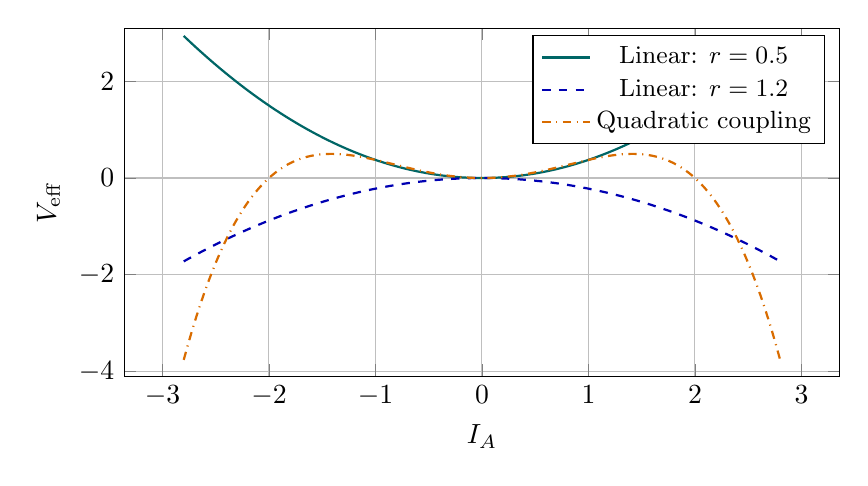
\begin{tikzpicture}
\begin{axis}[width=.88\textwidth,height=6cm,grid=major,legend style={font=\small},xlabel={$I_A$},ylabel={$V_{\mathrm{eff}}$},ymin=-4.1,ymax=3.1]
\addplot[teal!80!black,thick] coordinates{(-2.8,2.94) (-2.7626667,2.8621227) (-2.7253333,2.7852907) (-2.688,2.709504) (-2.6506667,2.6347627) (-2.6133333,2.5610667) (-2.576,2.488416) (-2.5386667,2.4168107) (-2.5013333,2.3462507) (-2.464,2.276736) (-2.4266667,2.2082667) (-2.3893333,2.1408427) (-2.352,2.074464) (-2.3146667,2.0091307) (-2.2773333,1.9448427) (-2.24,1.8816) (-2.2026667,1.8194027) (-2.1653333,1.7582507) (-2.128,1.698144) (-2.0906667,1.6390827) (-2.0533333,1.5810667) (-2.016,1.524096) (-1.9786667,1.4681707) (-1.9413333,1.4132907) (-1.904,1.359456) (-1.8666667,1.3066667) (-1.8293333,1.2549227) (-1.792,1.204224) (-1.7546667,1.1545707) (-1.7173333,1.1059627) (-1.68,1.0584) (-1.6426667,1.0118827) (-1.6053333,0.96641067) (-1.568,0.921984) (-1.5306667,0.87860267) (-1.4933333,0.83626667) (-1.456,0.794976) (-1.4186667,0.75473067) (-1.3813333,0.71553067) (-1.344,0.677376) (-1.3066667,0.64026667) (-1.2693333,0.60420267) (-1.232,0.569184) (-1.1946667,0.53521067) (-1.1573333,0.50228267) (-1.12,0.4704) (-1.0826667,0.43956267) (-1.0453333,0.40977067) (-1.008,0.381024) (-0.97066667,0.35332267) (-0.93333333,0.32666667) (-0.896,0.301056) (-0.85866667,0.27649067) (-0.82133333,0.25297067) (-0.784,0.230496) (-0.74666667,0.20906667) (-0.70933333,0.18868267) (-0.672,0.169344) (-0.63466667,0.15105067) (-0.59733333,0.13380267) (-0.56,0.1176) (-0.52266667,0.10244267) (-0.48533333,0.088330667) (-0.448,0.075264) (-0.41066667,0.063242667) (-0.37333333,0.052266667) (-0.336,0.042336) (-0.29866667,0.033450667) (-0.26133333,0.025610667) (-0.224,0.018816) (-0.18666667,0.013066667) (-0.14933333,0.0083626667) (-0.112,0.004704) (-0.074666667,0.0020906667) (-0.037333333,0.00052266667) (0,0) (0.037333333,0.00052266667) (0.074666667,0.0020906667) (0.112,0.004704) (0.14933333,0.0083626667) (0.18666667,0.013066667) (0.224,0.018816) (0.26133333,0.025610667) (0.29866667,0.033450667) (0.336,0.042336) (0.37333333,0.052266667) (0.41066667,0.063242667) (0.448,0.075264) (0.48533333,0.088330667) (0.52266667,0.10244267) (0.56,0.1176) (0.59733333,0.13380267) (0.63466667,0.15105067) (0.672,0.169344) (0.70933333,0.18868267) (0.74666667,0.20906667) (0.784,0.230496) (0.82133333,0.25297067) (0.85866667,0.27649067) (0.896,0.301056) (0.93333333,0.32666667) (0.97066667,0.35332267) (1.008,0.381024) (1.0453333,0.40977067) (1.0826667,0.43956267) (1.12,0.4704) (1.1573333,0.50228267) (1.1946667,0.53521067) (1.232,0.569184) (1.2693333,0.60420267) (1.3066667,0.64026667) (1.344,0.677376) (1.3813333,0.71553067) (1.4186667,0.75473067) (1.456,0.794976) (1.4933333,0.83626667) (1.5306667,0.87860267) (1.568,0.921984) (1.6053333,0.96641067) (1.6426667,1.0118827) (1.68,1.0584) (1.7173333,1.1059627) (1.7546667,1.1545707) (1.792,1.204224) (1.8293333,1.2549227) (1.8666667,1.3066667) (1.904,1.359456) (1.9413333,1.4132907) (1.9786667,1.4681707) (2.016,1.524096) (2.0533333,1.5810667) (2.0906667,1.6390827) (2.128,1.698144) (2.1653333,1.7582507) (2.2026667,1.8194027) (2.24,1.8816) (2.2773333,1.9448427) (2.3146667,2.0091307) (2.352,2.074464) (2.3893333,2.1408427) (2.4266667,2.2082667) (2.464,2.276736) (2.5013333,2.3462507) (2.5386667,2.4168107) (2.576,2.488416) (2.6133333,2.5610667) (2.6506667,2.6347627) (2.688,2.709504) (2.7253333,2.7852907) (2.7626667,2.8621227) (2.8,2.94)};
\addlegendentry{Linear: $r=0.5$}
\addplot[blue!70!black,dashed,thick] coordinates{(-2.8,-1.7248) (-2.7626667,-1.679112) (-2.7253333,-1.6340372) (-2.688,-1.5895757) (-2.6506667,-1.5457274) (-2.6133333,-1.5024924) (-2.576,-1.4598707) (-2.5386667,-1.4178623) (-2.5013333,-1.3764671) (-2.464,-1.3356851) (-2.4266667,-1.2955164) (-2.3893333,-1.255961) (-2.352,-1.2170189) (-2.3146667,-1.17869) (-2.2773333,-1.1409744) (-2.24,-1.103872) (-2.2026667,-1.0673829) (-2.1653333,-1.0315071) (-2.128,-0.99624448) (-2.0906667,-0.96159516) (-2.0533333,-0.92755911) (-2.016,-0.89413632) (-1.9786667,-0.86132679) (-1.9413333,-0.82913052) (-1.904,-0.79754752) (-1.8666667,-0.76657778) (-1.8293333,-0.7362213) (-1.792,-0.70647808) (-1.7546667,-0.67734812) (-1.7173333,-0.64883143) (-1.68,-0.620928) (-1.6426667,-0.59363783) (-1.6053333,-0.56696092) (-1.568,-0.54089728) (-1.5306667,-0.5154469) (-1.4933333,-0.49060978) (-1.456,-0.46638592) (-1.4186667,-0.44277532) (-1.3813333,-0.41977799) (-1.344,-0.39739392) (-1.3066667,-0.37562311) (-1.2693333,-0.35446556) (-1.232,-0.33392128) (-1.1946667,-0.31399026) (-1.1573333,-0.2946725) (-1.12,-0.275968) (-1.0826667,-0.25787676) (-1.0453333,-0.24039879) (-1.008,-0.22353408) (-0.97066667,-0.20728263) (-0.93333333,-0.19164444) (-0.896,-0.17661952) (-0.85866667,-0.16220786) (-0.82133333,-0.14840946) (-0.784,-0.13522432) (-0.74666667,-0.12265244) (-0.70933333,-0.11069383) (-0.672,-0.09934848) (-0.63466667,-0.088616391) (-0.59733333,-0.078497564) (-0.56,-0.068992) (-0.52266667,-0.060099698) (-0.48533333,-0.051820658) (-0.448,-0.04415488) (-0.41066667,-0.037102364) (-0.37333333,-0.030663111) (-0.336,-0.02483712) (-0.29866667,-0.019624391) (-0.26133333,-0.015024924) (-0.224,-0.01103872) (-0.18666667,-0.0076657778) (-0.14933333,-0.0049060978) (-0.112,-0.00275968) (-0.074666667,-0.0012265244) (-0.037333333,-0.00030663111) (0,-0) (0.037333333,-0.00030663111) (0.074666667,-0.0012265244) (0.112,-0.00275968) (0.14933333,-0.0049060978) (0.18666667,-0.0076657778) (0.224,-0.01103872) (0.26133333,-0.015024924) (0.29866667,-0.019624391) (0.336,-0.02483712) (0.37333333,-0.030663111) (0.41066667,-0.037102364) (0.448,-0.04415488) (0.48533333,-0.051820658) (0.52266667,-0.060099698) (0.56,-0.068992) (0.59733333,-0.078497564) (0.63466667,-0.088616391) (0.672,-0.09934848) (0.70933333,-0.11069383) (0.74666667,-0.12265244) (0.784,-0.13522432) (0.82133333,-0.14840946) (0.85866667,-0.16220786) (0.896,-0.17661952) (0.93333333,-0.19164444) (0.97066667,-0.20728263) (1.008,-0.22353408) (1.0453333,-0.24039879) (1.0826667,-0.25787676) (1.12,-0.275968) (1.1573333,-0.2946725) (1.1946667,-0.31399026) (1.232,-0.33392128) (1.2693333,-0.35446556) (1.3066667,-0.37562311) (1.344,-0.39739392) (1.3813333,-0.41977799) (1.4186667,-0.44277532) (1.456,-0.46638592) (1.4933333,-0.49060978) (1.5306667,-0.5154469) (1.568,-0.54089728) (1.6053333,-0.56696092) (1.6426667,-0.59363783) (1.68,-0.620928) (1.7173333,-0.64883143) (1.7546667,-0.67734812) (1.792,-0.70647808) (1.8293333,-0.7362213) (1.8666667,-0.76657778) (1.904,-0.79754752) (1.9413333,-0.82913052) (1.9786667,-0.86132679) (2.016,-0.89413632) (2.0533333,-0.92755911) (2.0906667,-0.96159516) (2.128,-0.99624448) (2.1653333,-1.0315071) (2.2026667,-1.0673829) (2.24,-1.103872) (2.2773333,-1.1409744) (2.3146667,-1.17869) (2.352,-1.2170189) (2.3893333,-1.255961) (2.4266667,-1.2955164) (2.464,-1.3356851) (2.5013333,-1.3764671) (2.5386667,-1.4178623) (2.576,-1.4598707) (2.6133333,-1.5024924) (2.6506667,-1.5457274) (2.688,-1.5895757) (2.7253333,-1.6340372) (2.7626667,-1.679112) (2.8,-1.7248)};
\addlegendentry{Linear: $r=1.2$}
\addplot[orange!85!black,dashdotted,thick] coordinates{(-2.8,-3.7632) (-2.7626667,-3.4653886) (-2.7253333,-3.1821405) (-2.688,-2.9130275) (-2.6506667,-2.6576269) (-2.6133333,-2.4155222) (-2.576,-2.1863024) (-2.5386667,-1.9695625) (-2.5013333,-1.7649033) (-2.464,-1.5719314) (-2.4266667,-1.3902593) (-2.3893333,-1.2195052) (-2.352,-1.0592932) (-2.3146667,-0.90925337) (-2.2773333,-0.76902133) (-2.24,-0.63823872) (-2.2026667,-0.51655295) (-2.1653333,-0.40361725) (-2.128,-0.29909071) (-2.0906667,-0.20263821) (-2.0533333,-0.11393049) (-2.016,-0.032644104) (-1.9786667,0.041538572) (-1.9413333,0.10892933) (-1.904,0.16983412) (-1.8666667,0.22455309) (-1.8293333,0.27338053) (-1.792,0.31660494) (-1.7546667,0.35450896) (-1.7173333,0.3873694) (-1.68,0.41545728) (-1.6426667,0.43903775) (-1.6053333,0.45837015) (-1.568,0.473708) (-1.5306667,0.48529898) (-1.4933333,0.49338494) (-1.456,0.49820192) (-1.4186667,0.49998011) (-1.3813333,0.49894388) (-1.344,0.49531178) (-1.3066667,0.48929653) (-1.2693333,0.48110501) (-1.232,0.47093829) (-1.1946667,0.45899159) (-1.1573333,0.44545433) (-1.12,0.43051008) (-1.0826667,0.41433659) (-1.0453333,0.39710578) (-1.008,0.37898374) (-0.97066667,0.36013075) (-0.93333333,0.34070123) (-0.896,0.32084381) (-0.85866667,0.30070125) (-0.82133333,0.28041053) (-0.784,0.26010275) (-0.74666667,0.23990323) (-0.70933333,0.21993142) (-0.672,0.20030099) (-0.63466667,0.18111973) (-0.59733333,0.16248964) (-0.56,0.14450688) (-0.52266667,0.12726178) (-0.48533333,0.11083884) (-0.448,0.095316738) (-0.41066667,0.080768325) (-0.37333333,0.067260618) (-0.336,0.054854812) (-0.29866667,0.043606269) (-0.26133333,0.033564528) (-0.224,0.024773296) (-0.18666667,0.017270455) (-0.14933333,0.011088058) (-0.112,0.006252331) (-0.074666667,0.0027836703) (-0.037333333,0.00069664606) (0,0) (0.037333333,0.00069664606) (0.074666667,0.0027836703) (0.112,0.006252331) (0.14933333,0.011088058) (0.18666667,0.017270455) (0.224,0.024773296) (0.26133333,0.033564528) (0.29866667,0.043606269) (0.336,0.054854812) (0.37333333,0.067260618) (0.41066667,0.080768325) (0.448,0.095316738) (0.48533333,0.11083884) (0.52266667,0.12726178) (0.56,0.14450688) (0.59733333,0.16248964) (0.63466667,0.18111973) (0.672,0.20030099) (0.70933333,0.21993142) (0.74666667,0.23990323) (0.784,0.26010275) (0.82133333,0.28041053) (0.85866667,0.30070125) (0.896,0.32084381) (0.93333333,0.34070123) (0.97066667,0.36013075) (1.008,0.37898374) (1.0453333,0.39710578) (1.0826667,0.41433659) (1.12,0.43051008) (1.1573333,0.44545433) (1.1946667,0.45899159) (1.232,0.47093829) (1.2693333,0.48110501) (1.3066667,0.48929653) (1.344,0.49531178) (1.3813333,0.49894388) (1.4186667,0.49998011) (1.456,0.49820192) (1.4933333,0.49338494) (1.5306667,0.48529898) (1.568,0.473708) (1.6053333,0.45837015) (1.6426667,0.43903775) (1.68,0.41545728) (1.7173333,0.3873694) (1.7546667,0.35450896) (1.792,0.31660494) (1.8293333,0.27338053) (1.8666667,0.22455309) (1.904,0.16983412) (1.9413333,0.10892933) (1.9786667,0.041538572) (2.016,-0.032644104) (2.0533333,-0.11393049) (2.0906667,-0.20263821) (2.128,-0.29909071) (2.1653333,-0.40361725) (2.2026667,-0.51655295) (2.24,-0.63823872) (2.2773333,-0.76902133) (2.3146667,-0.90925337) (2.352,-1.0592932) (2.3893333,-1.2195052) (2.4266667,-1.3902593) (2.464,-1.5719314) (2.5013333,-1.7649033) (2.5386667,-1.9695625) (2.576,-2.1863024) (2.6133333,-2.4155222) (2.6506667,-2.6576269) (2.688,-2.9130275) (2.7253333,-3.1821405) (2.7626667,-3.4653886) (2.8,-3.7632)};
\addlegendentry{Quadratic coupling}
\end{axis}
\end{tikzpicture}
\caption{Effective potentials for linear couplings with $r=0.5$ and $r=1.2$ ($\beta=1$), and for $\mu_1=I_A^2/2$, $\kappa_0=\gamma=1$, $\sigma_0=0$. The nonlinear potential has a local well and maxima at $\pm\sqrt2$ but tends to negative infinity. These are potentials minimized over the other coordinates, not exact one-coordinate dynamical trajectories.}
\end{figure}
\section{Periodically prescribed geometry}
The autonomous energy bound does not automatically survive time-dependent geometry. For linear functions prescribe a fixed direction of the coupling vector:

\begin{equation}
a(\tau)=r(\tau)\cos\chi,\quad b(\tau)=r(\tau)\sin\chi,
\end{equation}
\begin{equation}
r(\tau)=r_0+\epsilon\cos(\Omega\tau),\quad 0<\epsilon<r_0,\quad r_0+\epsilon<1.
\end{equation}
The eigenvectors stay constant, so the soft mode decouples exactly:

\begin{equation}
\ddot\eta_-+[1-r_0-\epsilon\cos(\Omega\tau)]\eta_-=0.
\end{equation}
This is realizable in the identity reduction by $b=0$, positive $g_1$, and prescribed $\kappa(\tau)^2=\sqrt{\beta\gamma}\,r(\tau)/g_1$. It does not establish that full worldline dynamics generates this curvature. Rotating the coupling direction would introduce modal-basis derivative terms and invalidate this scalar reduction.

Substituting $z=\Omega\tau/2$ gives the standard Mathieu equation \cite{r12}:

\begin{equation}
\frac{d^2\eta_-}{dz^2}+[a_M-2q_M\cos(2z)]\eta_-=0,
\end{equation}
\begin{equation}
a_M=\frac{4(1-r_0)}{\Omega^2},\qquad q_M=\frac{2\epsilon}{\Omega^2}.
\end{equation}
Instantaneous positive stiffness does not guarantee bounded driven motion. Set $r_0=0.5$, $\epsilon=0.1$, $\Omega=\sqrt2$: $r$ stays in $[0.4,0.6]$, with $a_M=1$, $q_M=0.1$. Fundamental-matrix integration over one drive period $P=2\pi/\Omega$ gives

\begin{equation}
\operatorname{tr}{\cal M}=-2.0246669154,\qquad\det{\cal M}\simeq1,
\end{equation}
\begin{equation}
\rho_-=-0.8547928928,\quad \rho_+=-1.1698740226.
\end{equation}
These are Floquet multipliers. Unit determinant follows analytically from the zero trace of the first-order coefficient matrix. The computed trace is separated from -2 by much more than integration error. One multiplier has magnitude above one, giving envelope growth rate

\begin{equation}
\nu=\frac{\log|\rho_+|}{P}=0.0353140230.
\end{equation}
For a comparison drive $\Omega=2.2$, the same $r_0,\epsilon$ give multipliers approximately $-0.4369942829\pm0.8994642832\,i$, distinct and on the unit circle. This case is bounded by the periodic linear-system criterion. Both cases have positive instantaneous stiffness throughout. Figure 4 uses matched initial conditions.

\begin{figure}[htbp]\centering
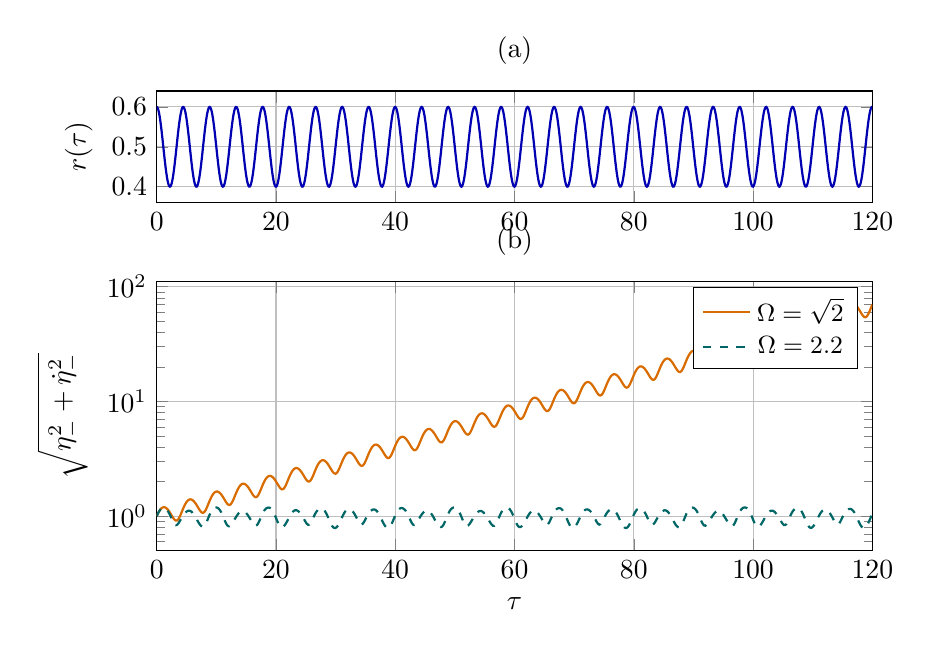
\begin{tikzpicture}
\begin{groupplot}[group style={group size=1 by 2,vertical sep=1cm},width=.88\textwidth,height=5cm,grid=major,xmin=0,xmax=120]
\nextgroupplot[ylabel={$r(\tau)$},title={(a)},ymin=.36,ymax=.64,height=3cm]
\addplot[blue!70!black,thick] coordinates{(0,0.6) (0.1,0.59900167) (0.2,0.5960266) (0.3,0.59113419) (0.4,0.58442214) (0.5,0.57602446) (0.6,0.56610882) (0.7,0.55487321) (0.8,0.54254196) (0.9,0.52936129) (1,0.51559437) (1.1,0.50151608) (1.2,0.48740752) (1.3,0.4735504) (1.4,0.46022138) (1.5,0.44768661) (1.6,0.43619637) (1.7,0.42598007) (1.8,0.41724171) (1.9,0.41015575) (2,0.40486369) (2.1,0.40147118) (2.2,0.40004597) (2.3,0.40061651) (2.4,0.40317141) (2.5,0.40765965) (2.6,0.41399163) (2.7,0.42204091) (2.8,0.43164677) (2.9,0.44261742) (3,0.45473381) (3.1,0.46775402) (3.2,0.48141807) (3.3,0.49545315) (3.4,0.509579) (3.5,0.5235136) (3.6,0.53697871) (3.7,0.54970547) (3.8,0.56143979) (3.9,0.57194735) (4,0.58101836) (4.1,0.5884717) (4.2,0.59415856) (4.3,0.59796538) (4.4,0.59981616) (4.5,0.59967394) (4.6,0.59754156) (4.7,0.5934616) (4.8,0.58751552) (4.9,0.57982205) (5,0.57053479) (5.1,0.55983919) (5.2,0.54794879) (5.3,0.53510102) (5.4,0.5215524) (5.5,0.50757345) (5.6,0.49344328) (5.7,0.47944402) (5.8,0.4658552) (5.9,0.45294814) (6,0.44098055) (6.1,0.43019138) (6.2,0.42079606) (6.3,0.41298218) (6.4,0.40690576) (6.5,0.40268812) (6.6,0.40041348) (6.7,0.40012725) (6.8,0.40183515) (6.9,0.40550307) (7,0.41105779) (7.1,0.41838839) (7.2,0.4273485) (7.3,0.43775922) (7.4,0.44941268) (7.5,0.46207621) (7.6,0.47549694) (7.7,0.48940693) (7.8,0.50352842) (7.9,0.51757946) (8,0.53127949) (8.1,0.54435498) (8.2,0.55654485) (8.3,0.5676057) (8.4,0.57731669) (8.5,0.58548393) (8.6,0.59194433) (8.7,0.59656891) (8.8,0.59926532) (8.9,0.59997974) (9,0.59869789) (9.1,0.59544537) (9.2,0.59028713) (9.3,0.58332615) (9.4,0.57470142) (9.5,0.56458515) (9.6,0.55317933) (9.7,0.5407117) (9.8,0.52743119) (9.9,0.51360296) (10,0.49950313) (10.1,0.48541323) (10.2,0.47161457) (10.3,0.45838267) (10.4,0.44598174) (10.5,0.43465937) (10.6,0.42464164) (10.7,0.41612856) (10.8,0.40929012) (10.9,0.40426285) (11,0.40114714) (11.1,0.40000519) (11.2,0.40085981) (11.3,0.40369393) (11.4,0.40845096) (11.5,0.41503593) (11.6,0.42331734) (11.7,0.43312986) (11.8,0.44427755) (11.9,0.45653783) (12,0.46966591) (12.1,0.48339966) (12.2,0.49746486) (12.3,0.51158068) (12.4,0.52546527) (12.5,0.53884141) (12.6,0.55144201) (12.7,0.56301549) (12.8,0.57333075) (12.9,0.58218184) (13,0.58939204) (13.1,0.59481737) (13.2,0.59834951) (13.3,0.59991794) (13.4,0.59949133) (13.5,0.59707822) (13.6,0.59272677) (13.7,0.58652388) (13.8,0.57859339) (13.9,0.56909365) (14,0.55821434) (14.1,0.54617269) (14.2,0.53320911) (14.3,0.51958246) (14.4,0.50556482) (14.5,0.49143606) (14.6,0.4774783) (14.7,0.46397022) (14.8,0.45118154) (14.9,0.43936759) (15,0.42876428) (15.1,0.41958331) (15.2,0.412008) (15.3,0.40618959) (15.4,0.40224426) (15.5,0.4002508) (15.6,0.40024899) (15.7,0.40223889) (15.8,0.40618075) (15.9,0.41199587) (16,0.41956814) (16.1,0.42874636) (16.2,0.43934729) (16.3,0.45115925) (16.4,0.4639464) (16.5,0.47745342) (16.6,0.49141062) (16.7,0.50553932) (16.8,0.51955742) (16.9,0.53318503) (17,0.54615003) (17.1,0.55819358) (17.2,0.56907519) (17.3,0.5785776) (17.4,0.58651107) (17.5,0.59271721) (17.6,0.59707209) (17.7,0.59948876) (17.8,0.59991897) (17.9,0.59835413) (18,0.59482548) (18.1,0.58940348) (18.2,0.58219639) (18.3,0.57334811) (18.4,0.56303531) (18.5,0.55146391) (18.6,0.53886494) (18.7,0.52548997) (18.8,0.51160604) (18.9,0.49749039) (19,0.48342484) (19.1,0.46969024) (19.2,0.45656083) (19.3,0.44429875) (19.4,0.43314885) (19.5,0.42333374) (19.6,0.4150494) (19.7,0.40846124) (19.8,0.40370081) (19.9,0.40086316) (20,0.40000494) (20.1,0.40114329) (20.2,0.40425548) (20.3,0.40927937) (20.4,0.41611466) (20.5,0.42462485) (20.6,0.43464004) (20.7,0.44596025) (20.8,0.45835945) (20.9,0.47159008) (21,0.48538796) (21.1,0.4994776) (21.2,0.51357766) (21.3,0.52740663) (21.4,0.54068837) (21.5,0.5531577) (21.6,0.56456565) (21.7,0.57468444) (21.8,0.58331203) (21.9,0.59027615) (22,0.59543775) (22.1,0.59869378) (22.2,0.59997922) (22.3,0.59926841) (22.4,0.59657553) (22.5,0.59195437) (22.6,0.58549717) (22.7,0.57733289) (22.8,0.56762452) (22.9,0.55656591) (23,0.54437787) (23.1,0.53130375) (23.2,0.5176046) (23.3,0.50355394) (23.4,0.48943232) (23.5,0.4755217) (23.6,0.46209984) (23.7,0.44943471) (23.8,0.43777921) (23.9,0.42736605) (24,0.41840314) (24.1,0.41106946) (24.2,0.40551143) (24.3,0.40184002) (24.4,0.40012854) (24.5,0.40041116) (24.6,0.40268224) (24.7,0.40689644) (24.8,0.4129696) (24.9,0.42078048) (25,0.4301731) (25.1,0.44095994) (25.2,0.45292561) (25.3,0.4658312) (25.4,0.47941903) (25.5,0.49341779) (25.6,0.50754798) (25.7,0.52152746) (25.8,0.53507711) (25.9,0.54792638) (26,0.55981873) (26.1,0.57051669) (26.2,0.57980666) (26.3,0.58750316) (26.4,0.59345252) (26.5,0.59753593) (26.6,0.59967188) (26.7,0.59981771) (26.8,0.59797051) (26.9,0.59416716) (27,0.5884836) (27.1,0.58103333) (27.2,0.57196508) (27.3,0.56145993) (27.4,0.54972763) (27.5,0.53700243) (27.6,0.52353842) (27.7,0.50960442) (27.8,0.49547866) (27.9,0.48144317) (28,0.46777819) (28.1,0.45475659) (28.2,0.44263834) (28.3,0.43166541) (28.4,0.4220569) (28.5,0.41400466) (28.6,0.40766946) (28.7,0.40317779) (28.8,0.40061934) (28.9,0.4000452) (29,0.40146682) (29.1,0.40485582) (29.2,0.41014454) (29.3,0.41722737) (29.4,0.4259629) (29.5,0.43617671) (29.6,0.44766485) (29.7,0.46019795) (29.8,0.47352577) (29.9,0.48738219) (30,0.50149055) (30.1,0.51556915) (30.2,0.52933688) (30.3,0.54251885) (30.4,0.55485186) (30.5,0.56608966) (30.6,0.57600787) (30.7,0.58440845) (30.8,0.59112368) (30.9,0.59601947) (31,0.59899806) (31.1,0.6) (31.2,0.59900526) (31.3,0.59603372) (31.4,0.5911447) (31.5,0.58443583) (31.6,0.57604105) (31.7,0.56612798) (31.8,0.55489455) (31.9,0.54256507) (32,0.5293857) (32.1,0.51561959) (32.2,0.50154162) (32.3,0.48743286) (32.4,0.47357502) (32.5,0.46024481) (32.6,0.44770838) (32.7,0.43621603) (32.8,0.42599724) (32.9,0.41725604) (33,0.41016697) (33.1,0.40487156) (33.2,0.40147555) (33.3,0.40004675) (33.4,0.40061368) (33.5,0.40316503) (33.6,0.40764986) (33.7,0.41397861) (33.8,0.42202492) (33.9,0.43162813) (34,0.44259651) (34.1,0.45471105) (34.2,0.46772985) (34.3,0.48139298) (34.4,0.49542764) (34.5,0.50955358) (34.6,0.52348878) (34.7,0.53695498) (34.8,0.54968331) (34.9,0.56141964) (35,0.57192961) (35.1,0.58100339) (35.2,0.5884598) (35.3,0.59414996) (35.4,0.59796026) (35.5,0.59981461) (35.6,0.599676) (35.7,0.59754719) (35.8,0.59347068) (35.9,0.58752787) (36,0.57983743) (36.1,0.57055289) (36.2,0.55985965) (36.3,0.5479712) (36.4,0.53512493) (36.5,0.52157733) (36.6,0.50759891) (36.7,0.49346876) (36.8,0.47946901) (36.9,0.46587921) (37,0.45297068) (37.1,0.44100117) (37.2,0.43020967) (37.3,0.42081165) (37.4,0.41299477) (37.5,0.40691509) (37.6,0.402694) (37.7,0.4004158) (37.8,0.40012596) (37.9,0.40183028) (38,0.40549472) (38.1,0.41104612) (38.2,0.41837363) (38.3,0.42733095) (38.4,0.43773923) (38.5,0.44939066) (38.6,0.46205258) (38.7,0.47547219) (38.8,0.48938153) (38.9,0.5035029) (39,0.51755432) (39.1,0.53125524) (39.2,0.54433209) (39.3,0.55652379) (39.4,0.56758688) (39.5,0.5773005) (39.6,0.58547067) (39.7,0.59193428) (39.8,0.59656227) (39.9,0.59926223) (40,0.59998025) (40.1,0.598702) (40.2,0.59545299) (40.3,0.5902981) (40.4,0.58334026) (40.5,0.57471839) (40.6,0.56460465) (40.7,0.55320096) (40.8,0.54073502) (40.9,0.52745574) (41,0.51362826) (41.1,0.49952867) (41.2,0.48543849) (41.3,0.47163905) (41.4,0.45840589) (41.5,0.44600323) (41.6,0.4346787) (41.7,0.42465842) (41.8,0.41614247) (41.9,0.40930087) (42,0.40427023) (42.1,0.401151) (42.2,0.40000546) (42.3,0.40085647) (42.4,0.40368706) (42.5,0.40844069) (42.6,0.41502246) (42.7,0.42330096) (42.8,0.43311087) (42.9,0.44425634) (43,0.45651483) (43.1,0.46964157) (43.2,0.48337447) (43.3,0.49743933) (43.4,0.51155531) (43.5,0.52544058) (43.6,0.53881788) (43.7,0.55142011) (43.8,0.56299566) (43.9,0.57331339) (44,0.58216729) (44.1,0.58938059) (44.2,0.59480925) (44.3,0.59834488) (44.4,0.5999169) (44.5,0.5994939) (44.6,0.59708434) (44.7,0.59273633) (44.8,0.58653668) (44.9,0.57860918) (45,0.56911211) (45.1,0.5582351) (45.2,0.54619534) (45.3,0.5332332) (45.4,0.51960751) (45.5,0.50559032) (45.6,0.4914615) (45.7,0.47750318) (45.8,0.46399404) (45.9,0.45120382) (46,0.4393879) (46.1,0.42878221) (46.2,0.41959849) (46.3,0.41202013) (46.4,0.40619844) (46.5,0.40224965) (46.6,0.40025261) (46.7,0.4002472) (46.8,0.40223352) (46.9,0.40617191) (47,0.41198374) (47.1,0.41955296) (47.2,0.42872845) (47.3,0.43932699) (47.4,0.45113697) (47.5,0.46392258) (47.6,0.47742854) (47.7,0.49138518) (47.8,0.50551383) (47.9,0.51953238) (48,0.53316094) (48.1,0.54612738) (48.2,0.55817281) (48.3,0.56905672) (48.4,0.5785618) (48.5,0.58649826) (48.6,0.59270764) (48.7,0.59706595) (48.8,0.59948617) (48.9,0.59991999) (49,0.59835874) (49.1,0.59483358) (49.2,0.58941492) (49.3,0.58221093) (49.4,0.57336547) (49.5,0.56305513) (49.6,0.5514858) (49.7,0.53888847) (49.8,0.52551466) (49.9,0.51163141) (50,0.49751591) (50.1,0.48345002) (50.2,0.46971458) (50.3,0.45658383) (50.4,0.44431996) (50.5,0.43316784) (50.6,0.42335013) (50.7,0.41506287) (50.8,0.40847153) (50.9,0.4037077) (51,0.40086651) (51.1,0.40000469) (51.2,0.40113944) (51.3,0.40424811) (51.4,0.40926863) (51.5,0.41610076) (51.6,0.42460807) (51.7,0.43462071) (51.8,0.44593876) (51.9,0.45833624) (52,0.4715656) (52.1,0.4853627) (52.2,0.49945206) (52.3,0.51355236) (52.4,0.52738207) (52.5,0.54066504) (52.6,0.55313607) (52.7,0.56454615) (52.8,0.57466746) (52.9,0.5832979) (53,0.59026516) (53.1,0.59543012) (53.2,0.59868966) (53.3,0.5999787) (53.4,0.59927149) (53.5,0.59658216) (53.6,0.5919644) (53.7,0.58551042) (53.8,0.57734907) (53.9,0.56764333) (54,0.55658697) (54.1,0.54440075) (54.2,0.531328) (54.3,0.51762973) (54.4,0.50357946) (54.5,0.48945771) (54.6,0.47554646) (54.7,0.46212347) (54.8,0.44945674) (54.9,0.4377992) (55,0.4273836) (55.1,0.41841791) (55.2,0.41108114) (55.3,0.40551979) (55.4,0.4018449) (55.5,0.40012984) (55.6,0.40040885) (55.7,0.40267637) (55.8,0.40688712) (55.9,0.41295703) (56,0.4207649) (56.1,0.43015482) (56.2,0.44093933) (56.3,0.45290308) (56.4,0.4658072) (56.5,0.47939404) (56.6,0.49339231) (56.7,0.50752252) (56.8,0.52150252) (56.9,0.5350532) (57,0.54790397) (57.1,0.55979826) (57.2,0.57049858) (57.3,0.57979127) (57.4,0.5874908) (57.5,0.59344343) (57.6,0.5975303) (57.7,0.59966981) (57.8,0.59981924) (57.9,0.59797562) (58,0.59417575) (58.1,0.5884955) (58.2,0.58104829) (58.3,0.57198281) (58.4,0.56148007) (58.5,0.54974978) (58.6,0.53702615) (58.7,0.52356324) (58.8,0.50962984) (58.9,0.49550417) (59,0.48146826) (59.1,0.46780237) (59.2,0.45477936) (59.3,0.44265926) (59.4,0.43168406) (59.5,0.4220729) (59.6,0.4140177) (59.7,0.40767927) (59.8,0.40318418) (59.9,0.40062219) (60,0.40004443) (60.1,0.40146247) (60.2,0.40484797) (60.3,0.41013334) (60.4,0.41721305) (60.5,0.42594574) (60.6,0.43615705) (60.7,0.44764309) (60.8,0.46017453) (60.9,0.47350115) (61,0.48735686) (61.1,0.50146502) (61.2,0.51554392) (61.3,0.52931246) (61.4,0.54249573) (61.5,0.55483051) (61.6,0.56607049) (61.7,0.57599127) (61.8,0.58439476) (61.9,0.59111316) (62,0.59601233) (62.1,0.59899445) (62.2,0.59999999) (62.3,0.59900885) (62.4,0.59604084) (62.5,0.5911552) (62.6,0.5844495) (62.7,0.57605763) (62.8,0.56614713) (62.9,0.5549159) (63,0.54258817) (63.1,0.52941011) (63.2,0.51564481) (63.3,0.50156715) (63.4,0.48745819) (63.5,0.47359965) (63.6,0.46026824) (63.7,0.44773014) (63.8,0.4362357) (63.9,0.42601442) (64,0.41727038) (64.1,0.41017819) (64.2,0.40487943) (64.3,0.40147992) (64.4,0.40004753) (64.5,0.40061086) (64.6,0.40315866) (64.7,0.40764006) (64.8,0.41396559) (64.9,0.42200893) (65,0.4316095) (65.1,0.4425756) (65.2,0.45468828) (65.3,0.46770568) (65.4,0.48136789) (65.5,0.49540213) (65.6,0.50952816) (65.7,0.52346396) (65.8,0.53693125) (65.9,0.54966115) (66,0.56139948) (66.1,0.57191187) (66.2,0.58098841) (66.3,0.58844789) (66.4,0.59414135) (66.5,0.59795512) (66.6,0.59981305) (66.7,0.59967805) (66.8,0.5975528) (66.9,0.59347975) (67,0.58754022) (67.1,0.5798528) (67.2,0.57057098) (67.3,0.5598801) (67.4,0.54799361) (67.5,0.53514884) (67.6,0.52160227) (67.7,0.50762437) (67.8,0.49349424) (67.9,0.47949401) (68,0.46590321) (68.1,0.45299321) (68.2,0.44102179) (68.3,0.43022796) (68.4,0.42082725) (68.5,0.41300736) (68.6,0.40692442) (68.7,0.4026999) (68.8,0.40041813) (68.9,0.40012469) (69,0.40182542) (69.1,0.40548638) (69.2,0.41103445) (69.3,0.41835888) (69.4,0.42731341) (69.5,0.43771925) (69.6,0.44936863) (69.7,0.46202895) (69.8,0.47544743) (69.9,0.48935614) (70,0.50347738) (70.1,0.51752918) (70.2,0.53123098) (70.3,0.5443092) (70.4,0.55650272) (70.5,0.56756806) (70.6,0.57728429) (70.7,0.58545741) (70.8,0.59192423) (70.9,0.59655563) (71,0.59925913) (71.1,0.59998075) (71.2,0.59870609) (71.3,0.5954606) (71.4,0.59030907) (71.5,0.58335437) (71.6,0.57473536) (71.7,0.56462414) (71.8,0.55322258) (71.9,0.54075834) (72,0.52748029) (72.1,0.51365356) (72.2,0.49955421) (72.3,0.48546375) (72.4,0.47166354) (72.5,0.45842912) (72.6,0.44602472) (72.7,0.43469804) (72.8,0.42467522) (72.9,0.41615638) (73,0.40931163) (73.1,0.40427762) (73.2,0.40115487) (73.3,0.40000573) (73.4,0.40085314) (73.5,0.40368019) (73.6,0.40843043) (73.7,0.41500901) (73.8,0.42328457) (73.9,0.43309189) (74,0.44423515) (74.1,0.45649184) (74.2,0.46961724) (74.3,0.48334929) (74.4,0.4974138) (74.5,0.51152995) (74.6,0.52541588) (74.7,0.53879434) (74.8,0.55139821) (74.9,0.56297582) (75,0.57329602) (75.1,0.58215274) (75.2,0.58936913) (75.3,0.59480113) (75.4,0.59834025) (75.5,0.59991585) (75.6,0.59949646) (75.7,0.59709046) (75.8,0.59274588) (75.9,0.58654947) (76,0.57862496) (76.1,0.56913056) (76.2,0.55825586) (76.3,0.54621798) (76.4,0.53325728) (76.5,0.51963255) (76.6,0.50561581) (76.7,0.49148695) (76.8,0.47752806) (76.9,0.46401787) (77,0.45122611) (77.1,0.43940822) (77.2,0.42880013) (77.3,0.41961368) (77.4,0.41203227) (77.5,0.40620729) (77.6,0.40225504) (77.7,0.40025443) (77.8,0.40024541) (77.9,0.40222815) (78,0.40616308) (78.1,0.41197162) (78.2,0.4195378) (78.3,0.42871054) (78.4,0.43930669) (78.5,0.45111469) (78.6,0.46389877) (78.7,0.47740367) (78.8,0.49135974) (78.9,0.50548833) (79,0.51950733) (79.1,0.53313684) (79.2,0.54610472) (79.3,0.55815204) (79.4,0.56903825) (79.5,0.578546) (79.6,0.58648544) (79.7,0.59269806) (79.8,0.59705981) (79.9,0.59948359) (80,0.59992101) (80.1,0.59836334) (80.2,0.59484168) (80.3,0.58942635) (80.4,0.58222547) (80.5,0.57338282) (80.6,0.56307495) (80.7,0.55150769) (80.8,0.53891199) (80.9,0.52553935) (81,0.51165677) (81.1,0.49754144) (81.2,0.48347521) (81.3,0.46973891) (81.4,0.45660684) (81.5,0.44434118) (81.6,0.43318684) (81.7,0.42336654) (81.8,0.41507635) (81.9,0.40848181) (82,0.40371459) (82.1,0.40086987) (82.2,0.40000444) (82.3,0.4011356) (82.4,0.40424075) (82.5,0.4092579) (82.6,0.41608686) (82.7,0.4245913) (82.8,0.43460139) (82.9,0.44591728) (83,0.45831303) (83.1,0.47154112) (83.2,0.48533744) (83.3,0.49942653) (83.4,0.51352706) (83.5,0.52735751) (83.6,0.54064171) (83.7,0.55311444) (83.8,0.56452665) (83.9,0.57465047) (84,0.58328377) (84.1,0.59025417) (84.2,0.59542249) (84.3,0.59868554) (84.4,0.59997817) (84.5,0.59927456) (84.6,0.59658877) (84.7,0.59197443) (84.8,0.58552365) (84.9,0.57736526) (85,0.56766213) (85.1,0.55660802) (85.2,0.54442363) (85.3,0.53135225) (85.4,0.51765487) (85.5,0.50360498) (85.6,0.48948311) (85.7,0.47557122) (85.8,0.4621471) (85.9,0.44947878) (86,0.4378192) (86.1,0.42740116) (86.2,0.41843268) (86.3,0.41109283) (86.4,0.40552816) (86.5,0.40184978) (86.6,0.40013114) (86.7,0.40040655) (86.8,0.40267051) (86.9,0.40687781) (87,0.41294446) (87.1,0.42074932) (87.2,0.43013655) (87.3,0.44091873) (87.4,0.45288056) (87.5,0.46578321) (87.6,0.47936906) (87.7,0.49336683) (87.8,0.50749706) (87.9,0.52147758) (88,0.53502928) (88.1,0.54788155) (88.2,0.55977779) (88.3,0.57048047) (88.4,0.57977588) (88.5,0.58747843) (88.6,0.59343433) (88.7,0.59752465) (88.8,0.59966773) (88.9,0.59982078) (89,0.59798073) (89.1,0.59418433) (89.2,0.58850739) (89.3,0.58106324) (89.4,0.57200053) (89.5,0.56150021) (89.6,0.54977193) (89.7,0.53704987) (89.8,0.52358805) (89.9,0.50965526) (90,0.49552968) (90.1,0.48149335) (90.2,0.46782655) (90.3,0.45480214) (90.4,0.44268018) (90.5,0.43170271) (90.6,0.42208891) (90.7,0.41403074) (90.8,0.40768909) (90.9,0.40319058) (91,0.40062503) (91.1,0.40004368) (91.2,0.40145812) (91.3,0.40484011) (91.4,0.41012214) (91.5,0.41719873) (91.6,0.42592858) (91.7,0.4361374) (91.8,0.44762134) (91.9,0.46015111) (92,0.47347652) (92.1,0.48733153) (92.2,0.50143948) (92.3,0.51551869) (92.4,0.52928805) (92.5,0.54247262) (92.6,0.55480915) (92.7,0.56605132) (92.8,0.57597467) (92.9,0.58438106) (93,0.59110263) (93.1,0.59600519) (93.2,0.59899084) (93.3,0.59999997) (93.4,0.59901243) (93.5,0.59604795) (93.6,0.5911657) (93.7,0.58446318) (93.8,0.5760742) (93.9,0.56616628) (94,0.55493724) (94.1,0.54261128) (94.2,0.52943451) (94.3,0.51567004) (94.4,0.50159268) (94.5,0.48748353) (94.6,0.47362428) (94.7,0.46029168) (94.8,0.44775192) (94.9,0.43625537) (95,0.4260316) (95.1,0.41728473) (95.2,0.41018941) (95.3,0.40488732) (95.4,0.4014843) (95.5,0.40004832) (95.6,0.40060805) (95.7,0.4031523) (95.8,0.40763028) (95.9,0.41395257) (96,0.42199295) (96.1,0.43159087) (96.2,0.4425547) (96.3,0.45466552) (96.4,0.46768151) (96.5,0.48134281) (96.6,0.49537662) (96.7,0.50950274) (96.8,0.52343913) (96.9,0.53690752) (97,0.54963898) (97.1,0.56137932) (97.2,0.57189412) (97.3,0.58097343) (97.4,0.58843597) (97.5,0.59413273) (97.6,0.59794998) (97.7,0.59981149) (97.8,0.59968009) (97.9,0.59755842) (98,0.59348882) (98.1,0.58755256) (98.2,0.57986817) (98.3,0.57058907) (98.4,0.55990055) (98.5,0.54801601) (98.6,0.53517275) (98.7,0.5216272) (98.8,0.50764983) (98.9,0.49351972) (99,0.479519) (99.1,0.46592722) (99.2,0.45301575) (99.3,0.44104241) (99.4,0.43024626) (99.5,0.42084285) (99.6,0.41301996) (99.7,0.40693376) (99.8,0.40270579) (99.9,0.40042047) (100,0.40012341) (100.1,0.40182057) (100.2,0.40547804) (100.3,0.4110228) (100.4,0.41834414) (100.5,0.42729588) (100.6,0.43769928) (100.7,0.44934661) (100.8,0.46200533) (100.9,0.47542268) (101,0.48933075) (101.1,0.50345186) (101.2,0.51750404) (101.3,0.53120672) (101.4,0.54428631) (101.5,0.55648165) (101.6,0.56754923) (101.7,0.57726809) (101.8,0.58544415) (101.9,0.59191418) (102,0.59654898) (102.1,0.59925602) (102.2,0.59998125) (102.3,0.59871019) (102.4,0.5954682) (102.5,0.59032004) (102.6,0.58336848) (102.7,0.57475233) (102.8,0.56464362) (102.9,0.55324419) (103,0.54078166) (103.1,0.52750485) (103.2,0.51367885) (103.3,0.49957974) (103.4,0.48548902) (103.5,0.47168803) (103.6,0.45845234) (103.7,0.44604622) (103.8,0.43471738) (103.9,0.42469202) (104,0.4161703) (104.1,0.40932239) (104.2,0.40428501) (104.3,0.40115874) (104.4,0.400006) (104.5,0.40084982) (104.6,0.40367333) (104.7,0.40842017) (104.8,0.41499555) (104.9,0.4232682) (105,0.43307292) (105.1,0.44421395) (105.2,0.45646885) (105.3,0.46959292) (105.4,0.48332411) (105.5,0.49738828) (105.6,0.51150458) (105.7,0.52539118) (105.8,0.5387708) (105.9,0.5513763) (106,0.56295598) (106.1,0.57327864) (106.2,0.58213817) (106.3,0.58935767) (106.4,0.594793) (106.5,0.59833562) (106.6,0.5999148) (106.7,0.59949902) (106.8,0.59709657) (106.9,0.59275543) (107,0.58656226) (107.1,0.57864073) (107.2,0.56914901) (107.3,0.55827661) (107.4,0.54624063) (107.5,0.53328136) (107.6,0.51965758) (107.7,0.50564131) (107.8,0.49151239) (107.9,0.47755295) (108,0.46404169) (108.1,0.45124841) (108.2,0.43942853) (108.3,0.42881807) (108.4,0.41962887) (108.5,0.41204442) (108.6,0.40621615) (108.7,0.40226043) (108.8,0.40025625) (108.9,0.40024362) (109,0.4022228) (109.1,0.40615426) (109.2,0.41195951) (109.3,0.41952264) (109.4,0.42869263) (109.5,0.4392864) (109.6,0.45109242) (109.7,0.46387495) (109.8,0.47737879) (109.9,0.4913343) (110,0.50546283) (110.1,0.51948229) (110.2,0.53311275) (110.3,0.54608206) (110.4,0.55813126) (110.5,0.56901977) (110.6,0.57853019) (110.7,0.58647262) (110.8,0.59268848) (110.9,0.59705366) (111,0.59948099) (111.1,0.59992202) (111.2,0.59836794) (111.3,0.59484977) (111.4,0.58943777) (111.5,0.58224) (111.6,0.57340016) (111.7,0.56309477) (111.8,0.55152958) (111.9,0.53893551) (112,0.52556404) (112.1,0.51168213) (112.2,0.49756697) (112.3,0.48350039) (112.4,0.46976325) (112.5,0.45662984) (112.6,0.44436239) (112.7,0.43320584) (112.8,0.42338295) (112.9,0.41508984) (113,0.40849211) (113.1,0.40372149) (113.2,0.40087323) (113.3,0.40000421) (113.4,0.40113177) (113.5,0.4042334) (113.6,0.40924717) (113.7,0.41607298) (113.8,0.42457453) (113.9,0.43458208) (114,0.44589581) (114.1,0.45828982) (114.2,0.47151664) (114.3,0.48531218) (114.4,0.49940099) (114.5,0.51350176) (114.6,0.52733294) (114.7,0.54061838) (114.8,0.5530928) (114.9,0.56450714) (115,0.57463347) (115.1,0.58326963) (115.2,0.59024317) (115.3,0.59541485) (115.4,0.59868141) (115.5,0.59997763) (115.6,0.59927763) (115.7,0.59659538) (115.8,0.59198445) (115.9,0.58553688) (116,0.57738143) (116.1,0.56768093) (116.2,0.55662907) (116.3,0.54444651) (116.4,0.5313765) (116.5,0.51768) (116.6,0.5036305) (116.7,0.4895085) (116.8,0.47559599) (116.9,0.46217074) (117,0.44950082) (117.1,0.4378392) (117.2,0.42741872) (117.3,0.41844746) (117.4,0.41110452) (117.5,0.40553654) (117.6,0.40185468) (117.7,0.40013245) (117.8,0.40040425) (117.9,0.40266465) (118,0.40686851) (118.1,0.4129319) (118.2,0.42073375) (118.3,0.43011828) (118.4,0.44089813) (118.5,0.45285804) (118.6,0.46575922) (118.7,0.47934407) (118.8,0.49334135) (118.9,0.50747159) (119,0.52145264) (119.1,0.53500536) (119.2,0.54785913) (119.3,0.55975732) (119.4,0.57046235) (119.5,0.57976048) (119.6,0.58746605) (119.7,0.59342522) (119.8,0.597519) (119.9,0.59966565) (120,0.5998223)};
\nextgroupplot[ylabel={$\sqrt{\eta_-^2+\dot\eta_-^2}$},xlabel={$\tau$},title={(b)},ymode=log,legend style={font=\small}]
\addplot[orange!85!black,thick] coordinates{(0,1) (0.2,1.0548843) (0.4,1.1043839) (0.6,1.1455241) (0.8,1.1761438) (1,1.1949294) (1.2,1.2014148) (1.4,1.1959291) (1.6,1.179483) (1.8,1.1536105) (2,1.1202184) (2.2,1.0815119) (2.4,1.0400472) (2.6,0.99889493) (2.8,0.96180586) (3,0.93317149) (3.2,0.91755414) (3.4,0.91872033) (3.6,0.93849007) (3.8,0.97603647) (4,1.0280753) (4.2,1.0897561) (4.4,1.1556901) (4.6,1.2207094) (4.8,1.2802927) (5,1.3307646) (5.2,1.3693884) (5.4,1.3944129) (5.6,1.405083) (5.8,1.4015932) (6,1.3849694) (6.2,1.3568912) (6.4,1.3195073) (6.6,1.2753231) (6.8,1.227228) (7,1.178666) (7.2,1.1338459) (7.4,1.0977701) (7.6,1.0758107) (7.8,1.0726896) (8,1.091123) (8.2,1.1308264) (8.4,1.1885047) (8.6,1.2587708) (8.8,1.3353663) (9,1.4121362) (9.2,1.4836027) (9.4,1.5452422) (9.6,1.5936114) (9.8,1.626412) (10,1.6425125) (10.2,1.6419111) (10.4,1.6256149) (10.6,1.5954442) (10.8,1.5538106) (11,1.5035591) (11.2,1.4479617) (11.4,1.3908862) (11.6,1.3370495) (11.8,1.2921239) (12,1.2623786) (12.2,1.2536307) (12.4,1.269688) (12.6,1.311016) (12.8,1.3744529) (13,1.4541003) (13.2,1.5427435) (13.4,1.6330842) (13.6,1.7185081) (13.8,1.7934674) (14,1.8536548) (14.2,1.8960905) (14.4,1.9191589) (14.6,1.9225827) (14.8,1.9073042) (15,1.8752709) (15.2,1.8291755) (15.4,1.7722456) (15.6,1.7081918) (15.8,1.6413647) (16,1.5770478) (16.2,1.5216484) (16.4,1.4824256) (16.6,1.4664404) (16.8,1.4788087) (17,1.5209933) (17.2,1.590157) (17.4,1.6799518) (17.6,1.7821299) (17.8,1.8880795) (18,1.9898414) (18.2,2.080635) (18.4,2.1550997) (18.6,2.2094106) (18.8,2.2413352) (19,2.2502209) (19.2,2.2368819) (19.4,2.2033695) (19.6,2.1526718) (19.8,2.0884436) (20,2.0148973) (20.2,1.9369357) (20.4,1.8604771) (20.6,1.7927369) (20.8,1.7420627) (21,1.7169168) (21.2,1.723961) (21.4,1.7659443) (21.6,1.840601) (21.8,1.941242) (22,2.0585279) (22.2,2.1823524) (22.4,2.3031723) (22.6,2.4127281) (22.8,2.5043778) (23,2.573254) (23.2,2.6163432) (23.4,2.6324926) (23.6,2.6223045) (23.8,2.587897) (24,2.5325606) (24.2,2.4604232) (24.4,2.3762699) (24.6,2.2856362) (24.8,2.1951554) (25,2.1129334) (25.2,2.0485128) (25.4,2.0119234) (25.6,2.0116309) (25.8,2.0520023) (26,2.1316543) (26.2,2.2437245) (26.4,2.3777533) (26.6,2.5219519) (26.8,2.6649226) (27,2.7966372) (27.2,2.9088996) (27.4,2.9955602) (27.6,3.0526245) (27.8,3.0782821) (28,3.072816) (28.2,3.0383547) (28.4,2.9784896) (28.6,2.8978663) (28.8,2.8019207) (29,2.6969142) (29.2,2.5902893) (29.4,2.4911373) (29.6,2.4103109) (29.8,2.3595827) (30,2.3495002) (30.2,2.3864248) (30.4,2.4702369) (30.6,2.5941423) (30.8,2.7465764) (31,2.9138809) (31.2,3.0825006) (31.4,3.2402991) (31.6,3.3772013) (31.8,3.485486) (32,3.5599329) (32.2,3.5978796) (32.4,3.5991499) (32.6,3.5658044) (32.8,3.5017198) (33,3.4121015) (33.2,3.3031208) (33.4,3.1818718) (33.6,3.056717) (33.8,2.9378428) (34,2.8375383) (34.2,2.7695045) (34.4,2.7466672) (34.6,2.7778034) (34.8,2.864516) (35,3.0004093) (35.2,3.17289) (35.4,3.366255) (35.6,3.5644566) (35.8,3.7528572) (36,3.9191151) (36.2,4.0535888) (36.4,4.1495344) (36.6,4.2031965) (36.8,4.2137623) (37,4.183117) (37.2,4.1153885) (37.4,4.0163778) (37.6,3.893082) (37.8,3.7535495) (38,3.6071924) (38.2,3.4654203) (38.4,3.3420988) (38.6,3.2530542) (38.8,3.2139059) (39,3.2363115) (39.2,3.3241388) (39.4,3.4718259) (39.6,3.6659083) (39.8,3.8884894) (40,4.1206668) (40.2,4.3448474) (40.4,4.5459647) (40.6,4.712037) (40.8,4.8344353) (41,4.9080145) (41.2,4.9311006) (41.4,4.9052596) (41.6,4.8348127) (41.8,4.7261818) (42,4.5872837) (42.2,4.427258) (42.4,4.2567181) (42.6,4.0884462) (42.8,3.9380427) (43,3.8236693) (43.2,3.7639722) (43.4,3.7739982) (43.6,3.8605102) (43.8,4.019336) (44,4.2364043) (44.2,4.4915212) (44.4,4.7625469) (44.6,5.0284146) (44.8,5.2707913) (45,5.4748528) (45.2,5.6296455) (45.4,5.7282708) (45.6,5.7679124) (45.8,5.7496278) (46,5.6778415) (46.2,5.5596061) (46.4,5.4038534) (46.6,5.2209661) (46.8,5.0229349) (47,4.8240907) (47.2,4.6419482) (47.4,4.4972313) (47.6,4.4119649) (47.8,4.4051349) (48,4.4871207) (48.2,4.6558333) (48.4,4.8969914) (48.6,5.1880712) (48.8,5.5033041) (49,5.8175637) (49.2,6.1086152) (49.4,6.3581903) (49.6,6.5524802) (49.8,6.6823871) (50,6.7436018) (50.2,6.7364277) (50.4,6.6652626) (50.6,6.5377768) (50.8,6.364009) (51,6.1557523) (51.2,5.9265777) (51.4,5.6925713) (51.6,5.4733693) (51.8,5.292504) (52,5.1757504) (52.2,5.1466249) (52.4,5.2199363) (52.6,5.3965247) (52.8,5.6624589) (53,5.9929554) (53.2,6.3582329) (53.4,6.7284532) (53.6,7.0767381) (53.8,7.3806575) (54,7.622907) (54.2,7.7916463) (54.4,7.8806382) (54.6,7.8891171) (54.8,7.8212725) (55,7.6853482) (55.2,7.4925735) (55.4,7.2563324) (55.6,6.9920081) (55.8,6.7176853) (56,6.455361) (56.2,6.2316479) (56.4,6.0764646) (56.6,6.0184868) (56.8,6.0778597) (57,6.2593631) (57.2,6.5501722) (57.4,6.923454) (57.6,7.3450647) (57.8,7.779738) (58,8.1950932) (58.2,8.5636862) (58.4,8.8639455) (58.6,9.0806266) (58.8,9.2050274) (59,9.2349138) (59.2,9.1740195) (59.4,9.0310765) (59.6,8.8185725) (59.8,8.5516732) (60,8.2478375) (60.2,7.9274325) (60.4,7.6150969) (60.6,7.3408267) (60.8,7.1391016) (61,7.0444252) (61.2,7.0832758) (61.4,7.2655612) (61.6,7.5805481) (61.8,7.9997504) (62,8.484379) (62.2,8.9929698) (62.4,9.4866521) (62.6,9.9319593) (62.8,10.302125) (63,10.577699) (63.2,10.746853) (63.4,10.805381) (63.6,10.756231) (63.8,10.608484) (64,10.375928) (64.2,10.075708) (64.4,9.7276532) (64.6,9.3547456) (64.8,8.9845933) (65,8.6509183) (65.2,8.3932091) (65.4,8.2525028) (65.6,8.2626974) (65.8,8.4402013) (66,8.7776216) (66.2,9.2454538) (66.4,9.8000914) (66.6,10.393068) (66.8,10.977898) (67,11.513904) (67.2,11.968015) (67.4,12.315602) (67.6,12.540899) (67.8,12.637099) (68,12.605936) (68.2,12.456625) (68.4,12.204262) (68.6,11.868167) (68.8,11.470868) (69,11.038343) (69.2,10.601558) (69.4,10.198352) (69.6,9.8737049) (69.8,9.6759332) (70,9.6475271) (70.2,9.8129589) (70.4,10.16972) (70.6,10.68822) (70.8,11.320031) (71,12.00887) (71.2,12.699374) (71.4,13.342262) (71.6,13.896831) (71.8,14.332095) (72,14.627365) (72.2,14.772445) (72.4,14.767301) (72.6,14.620978) (72.8,14.349833) (73,13.975549) (73.2,13.523708) (73.4,13.023729) (73.6,12.510387) (73.8,12.026089) (74,11.621838) (74.2,11.354015) (74.4,11.274958) (74.6,11.418959) (74.8,11.790265) (75,12.360492) (75.2,13.076625) (75.4,13.873786) (75.6,14.686329) (75.8,15.45475) (76,16.129133) (76.2,16.67072) (76.4,17.052686) (76.6,17.260481) (76.8,17.291589) (77,17.154466) (77.2,16.866614) (77.4,16.452241) (77.6,15.940368) (77.8,15.364358) (78,14.763328) (78.2,14.184779) (78.4,13.686321) (78.6,13.333233) (78.8,13.189037) (79,13.299792) (79.2,13.678723) (79.4,14.300379) (79.6,15.107713) (79.8,16.02656) (80,16.979465) (80.2,17.894826) (80.4,18.711639) (80.6,19.381666) (80.8,19.870482) (81,20.157981) (81.2,20.23827) (81.4,20.118647) (81.6,19.817546) (81.8,19.361828) (82,18.784354) (82.2,18.123001) (82.4,17.42185) (82.6,16.734111) (82.8,16.124656) (83,15.66855) (83.2,15.441915) (83.4,15.504712) (83.6,15.881742) (83.8,16.552709) (84,17.457513) (84.2,18.51218) (84.4,19.625817) (84.6,20.712577) (84.8,21.698151) (85,22.522773) (85.2,23.142637) (85.4,23.53061) (85.6,23.676292) (85.8,23.585076) (86,23.275988) (86.2,22.778608) (86.4,22.130048) (86.6,21.373336) (86.8,20.558241) (87,19.744403) (87.2,19.0047) (87.4,18.424937) (87.6,18.095327) (87.8,18.092058) (88,18.454489) (88.2,19.170274) (88.4,20.177773) (88.6,21.38295) (88.8,22.679786) (89,23.965754) (89.2,25.150634) (89.4,26.160681) (89.6,26.94055) (89.8,27.454282) (90,27.685557) (90.2,27.636888) (90.4,27.327392) (90.6,26.789349) (90.8,26.064528) (91,25.201805) (91.2,24.257479) (91.4,23.298464) (91.6,22.406497) (91.8,21.679161) (92,21.222336) (92.2,21.130928) (92.4,21.462243) (92.6,22.215316) (92.8,23.329141) (93,24.69976) (93.2,26.204349) (93.4,27.720977) (93.6,29.140462) (93.8,30.372154) (94,31.346567) (94.2,32.016713) (94.4,32.358602) (94.6,32.370611) (94.8,32.071241) (95,31.495331) (95.2,30.689681) (95.4,29.709781) (95.6,28.619417) (95.8,27.493775) (96,26.424439) (96.2,25.5219) (96.4,24.909377) (96.6,24.70316) (96.8,24.982283) (97,25.761295) (97.2,26.982795) (97.4,28.533595) (97.6,30.272491) (97.8,32.055139) (98,33.749858) (98.2,35.245609) (98.4,36.455628) (98.6,37.319216) (98.8,37.802549) (99,37.898267) (99.2,37.623288) (99.4,37.014705) (99.6,36.124668) (99.8,35.016092) (100,33.761344) (100.2,32.44505) (100.4,31.169788) (100.6,30.060224) (100.8,29.258679) (101,28.905662) (101.2,29.106119) (101.4,29.894986) (101.6,31.222386) (101.8,32.967326) (102,34.968886) (102.2,37.057056) (102.4,39.073571) (102.6,40.882877) (102.8,42.377161) (103,43.478758) (103.2,44.141335) (103.4,44.349785) (103.6,44.11814) (103.8,43.485226) (104,42.508771) (104.2,41.259959) (104.4,39.820968) (104.6,38.287226) (104.8,36.773652) (105,35.420508) (105.2,34.391107) (105.4,33.853172) (105.6,33.94213) (105.8,34.71897) (106,36.146348) (106.2,38.097844) (106.4,40.391897) (106.6,42.829389) (106.8,45.220814) (107,47.401234) (107.2,49.237261) (107.4,50.630317) (107.6,51.518287) (107.8,51.875779) (108,51.712242) (108.2,51.067422) (108.4,50.004712) (108.6,48.604419) (108.8,46.9599) (109,45.178968) (109.2,43.390466) (109.4,41.751866) (109.6,40.449511) (109.8,39.681499) (110,39.618683) (110.2,40.354592) (110.4,41.870653) (110.6,44.038592) (110.8,46.655926) (111,49.490911) (111.2,52.317532) (111.4,54.935753) (111.6,57.181201) (111.8,58.929606) (112,60.099067) (112.2,60.650751) (112.4,60.587312) (112.6,59.948247) (112.8,58.802493) (113,57.240305) (113.2,55.367724) (113.4,53.306771) (113.6,51.202074) (113.8,49.230175) (114,47.602663) (114.2,46.551349) (114.4,46.287822) (114.6,46.945464) (114.8,48.532079) (115,50.922589) (115.2,53.894224) (115.4,57.17917) (115.6,60.509037) (115.8,63.642023) (116,66.376315) (116.2,68.556192) (116.4,70.075073) (116.6,70.876771) (116.8,70.954316) (117,70.345311) (117.2,69.123845) (117.4,67.390872) (117.6,65.266733) (117.8,62.889749) (118,60.422517) (118.2,58.062804) (118.4,56.04989) (118.6,54.652831) (118.8,54.12961) (119,54.66161) (119.2,56.292106) (119.4,58.906022) (119.6,62.262203) (119.8,66.053627) (120,69.96309)};
\addlegendentry{$\Omega=\sqrt2$}
\addplot[teal!80!black,dashed,thick] coordinates{(0,1) (0.2,1.0547092) (0.4,1.103065) (0.6,1.141516) (0.8,1.1679796) (1,1.1818514) (1.2,1.1836081) (1.4,1.1741115) (1.6,1.1539908) (1.8,1.1235354) (2,1.0832358) (2.2,1.034673) (2.4,0.98123804) (2.6,0.9282741) (2.8,0.88244531) (3,0.85030604) (3.2,0.83633909) (3.4,0.8413412) (3.6,0.86230822) (3.8,0.89402539) (4,0.93121222) (4.2,0.96990202) (4.4,1.0076058) (4.6,1.0426442) (4.8,1.0733653) (5,1.097813) (5.2,1.1139462) (5.4,1.1201215) (5.6,1.115486) (5.8,1.1001367) (6,1.075102) (6.2,1.0422452) (6.4,1.0040966) (6.6,0.96354805) (6.8,0.9234202) (7,0.88611287) (7.2,0.85364702) (7.4,0.82816795) (7.6,0.81248708) (7.8,0.80996369) (8,0.82339729) (8.2,0.85349226) (8.4,0.89801381) (8.6,0.95221624) (8.8,1.0101) (9,1.0657306) (9.2,1.11422) (9.4,1.152295) (9.6,1.1784108) (9.8,1.1923721) (10,1.194583) (10.2,1.1853129) (10.4,1.1644376) (10.6,1.1318426) (10.8,1.0882332) (11,1.0358683) (11.2,0.9788513) (11.4,0.92285987) (11.6,0.87432677) (11.8,0.83911122) (12,0.82091541) (12.2,0.82018767) (12.4,0.83436207) (12.6,0.85938212) (12.8,0.89139504) (13,0.92755601) (13.2,0.96579389) (13.4,1.0041318) (13.6,1.0402469) (13.8,1.0715442) (14,1.09556) (14.2,1.110368) (14.4,1.1148175) (14.6,1.1086281) (14.8,1.0924194) (15,1.0676604) (15.2,1.0364507) (15.4,1.0011051) (15.6,0.96372799) (15.8,0.92612638) (16,0.89026656) (16.2,0.85903358) (16.4,0.83662637) (16.6,0.82792263) (16.8,0.83675059) (17,0.86398041) (17.2,0.90678184) (17.4,0.95951933) (17.6,1.0155069) (17.8,1.0686264) (18,1.1143475) (18.2,1.1500688) (18.4,1.1748132) (18.6,1.1884531) (18.8,1.1908768) (19,1.1815855) (19.2,1.1599509) (19.4,1.1259243) (19.6,1.0807358) (19.8,1.0272359) (20,0.96979261) (20.2,0.91382371) (20.4,0.86501796) (20.6,0.8282718) (20.8,0.80656815) (21,0.80037781) (21.2,0.80809653) (21.4,0.82725339) (21.6,0.8555517) (21.8,0.89107754) (22,0.93184718) (22.2,0.97534289) (22.4,1.0184829) (22.6,1.0579838) (22.8,1.0908185) (23,1.1145653) (23.2,1.1276337) (23.4,1.1294188) (23.6,1.1203567) (23.8,1.1017682) (24,1.0754383) (24.2,1.0430951) (24.4,1.0061629) (24.6,0.96609049) (24.8,0.92516268) (25,0.88726221) (25.2,0.85789225) (25.4,0.84300933) (25.6,0.84687887) (25.8,0.87008634) (26,0.9091066) (26.2,0.95769844) (26.4,1.0090427) (26.6,1.0574576) (26.8,1.0992074) (27,1.1324129) (27.2,1.1563198) (27.4,1.1703937) (27.6,1.173777) (27.8,1.1653931) (28,1.1445354) (28.2,1.1115129) (28.4,1.068005) (28.6,1.0170459) (28.8,0.96273953) (29,0.90980212) (29.2,0.86293531) (29.4,0.8260536) (29.6,0.80160597) (29.8,0.79041133) (30,0.79217244) (30.2,0.80622386) (30.4,0.83182465) (30.6,0.86780194) (30.8,0.91201918) (31,0.96123873) (31.2,1.0114917) (31.4,1.0586704) (31.6,1.0990623) (31.8,1.1297489) (32,1.1488983) (32.2,1.1559198) (32.4,1.1513611) (32.6,1.1364749) (32.8,1.1126067) (33,1.0807891) (33.2,1.0419093) (33.4,0.99745645) (33.6,0.95042513) (33.8,0.90577572) (34,0.8699717) (34.2,0.84942074) (34.4,0.84821829) (34.6,0.86638479) (34.8,0.89988215) (35,0.94241003) (35.2,0.98767798) (35.4,1.0309292) (35.6,1.0693191) (35.8,1.1013747) (36,1.1260836) (36.2,1.1422252) (36.4,1.1483091) (36.6,1.1430281) (36.8,1.1258375) (37,1.0973146) (37.2,1.0592078) (37.4,1.014272) (37.6,0.96599754) (37.8,0.91824093) (38,0.87472523) (38.2,0.83850881) (38.4,0.81170811) (38.6,0.79571091) (38.8,0.79169418) (39,0.80085248) (39.2,0.82392115) (39.4,0.86029022) (39.6,0.90747044) (39.8,0.96133867) (40,1.0169234) (40.2,1.0692612) (40.4,1.1140793) (40.6,1.14828) (40.8,1.17021) (41,1.179611) (41.2,1.1771769) (41.4,1.1638605) (41.6,1.1403251) (41.8,1.1069501) (42,1.0644642) (42.2,1.0148519) (42.4,0.96200343) (42.6,0.91170752) (42.8,0.87079849) (43,0.84547429) (43.2,0.8392416) (43.4,0.85159191) (43.6,0.87844808) (43.8,0.91412187) (44,0.95339736) (44.2,0.99261401) (44.4,1.029567) (44.6,1.0627285) (44.8,1.0905013) (45,1.1109904) (45.2,1.1223072) (45.4,1.1230735) (45.6,1.1127885) (45.8,1.0919441) (46,1.0619691) (46.2,1.0250966) (46.4,0.98415462) (46.6,0.94221774) (46.8,0.90216158) (47,0.86635668) (47.2,0.83679052) (47.4,0.8155984) (47.6,0.80549431) (47.8,0.80944255) (48,0.82944733) (48.2,0.8652134) (48.4,0.91369246) (48.6,0.96977295) (48.8,1.0275257) (49,1.0813638) (49.2,1.1268679) (49.4,1.1612416) (49.6,1.1833416) (49.8,1.1932387) (50,1.1914582) (50.2,1.1783055) (50.4,1.1537174) (50.6,1.1177646) (50.8,1.0714963) (51,1.017637) (51.2,0.96078843) (51.4,0.90702834) (51.6,0.86290719) (51.8,0.83391894) (52,0.8228663) (52.2,0.82904145) (52.4,0.84894543) (52.6,0.87809623) (52.8,0.91263558) (53,0.94986663) (53.2,0.98782451) (53.4,1.0245647) (53.6,1.0578) (53.8,1.0850577) (54,1.104113) (54.2,1.1133723) (54.4,1.1120699) (54.6,1.1003248) (54.8,1.0791358) (55,1.0502921) (55.2,1.0161137) (55.4,0.9790225) (55.6,0.94115989) (55.8,0.90439199) (56,0.87083969) (56.2,0.84359072) (56.4,0.8268821) (56.6,0.82518248) (56.8,0.8413655) (57,0.87509351) (57.2,0.92258386) (57.4,0.97780569) (57.6,1.0341854) (57.8,1.0860119) (58,1.1292579) (58.2,1.1617811) (58.4,1.1829288) (58.6,1.1927362) (58.8,1.1911416) (59,1.1776895) (59.2,1.1518929) (59.4,1.1139885) (59.6,1.0656162) (59.8,1.0100983) (60,0.95226005) (60.2,0.89785827) (60.4,0.85265999) (60.6,0.82123395) (60.8,0.80581791) (61,0.80595413) (61.2,0.8192776) (61.4,0.84290284) (61.6,0.87437547) (61.8,0.91170004) (62,0.95280524) (62.2,0.99512126) (62.4,1.0356248) (62.6,1.0712303) (62.8,1.0992226) (63,1.1175589) (63.2,1.1250528) (63.4,1.1214928) (63.6,1.1076568) (63.8,1.0851138) (64,1.0557815) (64.2,1.0214409) (64.4,0.98358319) (64.6,0.94384045) (64.8,0.90482056) (65,0.87074734) (65.2,0.84721434) (65.4,0.83971761) (65.6,0.85144195) (65.8,0.88163873) (66,0.9257729) (66.2,0.97722651) (66.4,1.0293456) (66.6,1.0768938) (66.8,1.1166259) (67,1.1470461) (67.2,1.1676133) (67.4,1.1778681) (67.6,1.1769904) (67.8,1.1640125) (68,1.1384649) (68.2,1.1010132) (68.4,1.0537651) (68.6,1.0001986) (68.8,0.94481837) (69,0.89261954) (69.2,0.84835742) (69.4,0.81569164) (69.6,0.79653555) (69.8,0.7910612) (70,0.79840314) (70.2,0.81746028) (70.4,0.84711724) (70.6,0.88584216) (70.8,0.93121447) (71,0.979884) (71.2,1.0279778) (71.4,1.0716548) (71.6,1.1075721) (71.8,1.1332263) (72,1.147201) (72.2,1.1492769) (72.4,1.1402815) (72.6,1.1216258) (72.8,1.0947158) (73,1.060635) (73.2,1.0204241) (73.4,0.97589228) (73.6,0.93047844) (73.8,0.88954127) (74,0.85961984) (74.2,0.8465962) (74.4,0.85341147) (74.6,0.87871656) (74.8,0.91748405) (75,0.96308849) (75.2,1.0094438) (75.4,1.0522276) (75.6,1.0890084) (75.8,1.1185761) (76,1.1400259) (76.2,1.1521789) (76.4,1.1536316) (76.6,1.1432769) (76.8,1.120885) (77,1.0874238) (77.2,1.0450605) (77.4,0.99695422) (77.6,0.94693835) (77.8,0.89908864) (78,0.85716288) (78.2,0.82405415) (78.4,0.80157556) (78.6,0.79076655) (78.8,0.79243122) (79,0.80729124) (79.2,0.83546304) (79.4,0.87568337) (79.6,0.92498726) (79.8,0.97908874) (80,1.0331496) (80.2,1.0825349) (80.4,1.1233948) (80.6,1.1530785) (80.8,1.1703446) (81,1.1752565) (81.2,1.1687002) (81.4,1.1517031) (81.6,1.1249653) (81.8,1.0889785) (82,1.0447425) (82.2,0.9946724) (82.4,0.94315667) (82.6,0.89637261) (82.8,0.86118183) (83,0.84321194) (83.2,0.84481499) (83.4,0.86416858) (83.6,0.89628524) (83.8,0.93520458) (84,0.97590613) (84.2,1.0150805) (84.4,1.0508013) (84.6,1.0816752) (84.8,1.1061544) (85,1.1224158) (85.2,1.128742) (85.4,1.1240388) (85.6,1.108169) (85.8,1.0820251) (86,1.0474351) (86.2,1.0069936) (86.4,0.96380731) (86.6,0.92110435) (86.8,0.88177987) (87,0.84813976) (87.2,0.82209859) (87.4,0.80571716) (87.6,0.80150361) (87.8,0.81190157) (88,0.83806125) (88.2,0.87876184) (88.4,0.93031131) (88.6,0.98739908) (88.8,1.0442705) (89,1.0957291) (89.2,1.1378286) (89.4,1.1682338) (89.6,1.1861762) (89.8,1.1919633) (90,1.1862201) (90.2,1.1692842) (90.4,1.1411702) (90.6,1.1021637) (90.8,1.0536894) (91,0.99895643) (91.2,0.94305681) (91.4,0.8924083) (91.6,0.85354138) (91.8,0.83138376) (92,0.82767041) (92.2,0.84051923) (92.4,0.86563232) (92.6,0.89827436) (92.8,0.93469627) (93,0.97239372) (93.2,1.0095165) (93.4,1.0441581) (93.6,1.0740821) (93.8,1.0969594) (94,1.1108231) (94.2,1.1144243) (94.4,1.1073872) (94.6,1.0902295) (94.8,1.0643216) (95,1.0317582) (95.2,0.99505956) (95.4,0.95673507) (95.6,0.91895188) (95.8,0.88363293) (96,0.85303976) (96.2,0.83039995) (96.4,0.81985072) (96.6,0.82527516) (96.8,0.8484923) (97,0.88802621) (97.2,0.93933464) (97.4,0.99618089) (97.6,1.0522175) (97.8,1.1021817) (98,1.1425474) (98.2,1.1716061) (98.4,1.1889975) (98.6,1.1948927) (98.8,1.1892694) (99,1.1717262) (99.2,1.1419428) (99.4,1.1004707) (99.6,1.0493827) (99.8,0.99248415) (100,0.93504327) (100.2,0.88309774) (100.4,0.84236915) (100.6,0.81692342) (100.8,0.80810321) (101,0.81448752) (101.2,0.83303558) (101.4,0.86057143) (101.6,0.89457701) (101.8,0.93303065) (102,0.97381234) (102.2,1.0143379) (102.4,1.051678) (102.6,1.0829715) (102.8,1.1058304) (103,1.1185966) (103.2,1.1204868) (103.4,1.1116746) (103.6,1.0932657) (103.8,1.0670575) (104,1.0350834) (104.2,0.99917147) (104.4,0.9608911) (104.6,0.92207537) (104.8,0.88565071) (105,0.85611378) (105.2,0.83899046) (105.4,0.83910995) (105.6,0.85845293) (105.8,0.8950038) (106,0.94342272) (106.2,0.99691493) (106.4,1.0491076) (106.6,1.0952463) (106.8,1.1325661) (107,1.1599233) (107.2,1.1769593) (107.4,1.1832733) (107.6,1.1780874) (107.8,1.1605628) (108,1.1304929) (108.2,1.0889221) (108.4,1.0384008) (108.6,0.98285318) (108.8,0.92716697) (109,0.87656316) (109.2,0.83574917) (109.4,0.80799312) (109.6,0.79455127) (109.8,0.79489524) (110,0.80761062) (110.2,0.8312167) (110.4,0.86429047) (110.6,0.90501688) (110.8,0.95077406) (111,0.99817442) (111.2,1.0434942) (111.4,1.0831873) (111.6,1.114291) (111.8,1.1347158) (112,1.1434518) (112.2,1.1406354) (112.4,1.1273523) (112.6,1.1051523) (112.8,1.0754938) (113,1.039522) (113.2,0.99845794) (113.4,0.95445624) (113.6,0.91139257) (113.8,0.87494738) (114,0.85156531) (114.2,0.84638326) (114.4,0.86105568) (114.6,0.89293005) (114.8,0.93619695) (115,0.98410535) (115.2,1.0308848) (115.4,1.0726764) (115.6,1.1074453) (115.8,1.1342138) (116,1.1521644) (116.2,1.1601589) (116.4,1.1568964) (116.6,1.141492) (116.8,1.1140504) (117,1.0759432) (117.2,1.0297616) (117.4,0.97906496) (117.6,0.92800874) (117.8,0.88084263) (118,0.84128575) (118.2,0.8119758) (118.4,0.79433713) (118.6,0.78899294) (118.8,0.79632408) (119,0.81655562) (119.2,0.84921626) (119.4,0.89248744) (119.6,0.94305912) (119.8,0.99659457) (120,1.0484569)};
\addlegendentry{$\Omega=2.2$}
\end{groupplot}
\end{tikzpicture}
\caption{Driven soft mode with $r_0=0.5$, $\epsilon=0.1$. Panel (a) shows resonant $r(\tau)$ below the static threshold. Panel (b) compares $\Omega=\sqrt2$ and $\Omega=2.2$ from the same state $(\eta_-,\dot\eta_-)=(0.8189831213,0.5738176079)$, a normalized growing Floquet eigenvector of the resonant case. The phase-space norm $\sqrt{\eta_-^2+\dot\eta_-^2}$ is displayed logarithmically. This is driven identity dynamics, not a demonstrated autonomous worldline instability.}
\end{figure}
The energy accounting is

\begin{equation}
H_R(\tau)=\frac12(|\dot X|^2+X^TB(\tau)X),\quad \dot H_R=\frac12X^T\dot B(\tau)X.
\end{equation}
The prescribed geometry does work on the identity sector, while $Q_O$ remains conserved. This separates subsystem conservation from static positive stiffness and from dynamical boundedness. Mathieu instability is established theory; the example demonstrates its relevance to this proposed coupling.

\section{Recurrence, reconstruction, and internal phase counters}
Return to constant geometry below threshold. The modal frequencies are

\begin{equation}
\omega_-=\sqrt{1-r},\quad \omega_0=1,\quad \omega_+=\sqrt{1+r}.
\end{equation}
Proposition 6. A linear solution exciting nonzero Origin is periodic in the full state $(I,\dot I)$ if and only if every excited modal frequency is rational relative to the unit Origin frequency.

Proof. A common period requires $T=2\pi n_O$, with positive integer $n_O$, and $\omega_jT=2\pi n_j$. Thus $\omega_j=n_j/n_O$. Conversely, common denominators give such an $n_O$. Zero-amplitude modes impose no condition. A return of coordinates without velocities is insufficient.

For $r=24/25$, the frequencies are $1/5,1,7/5$, giving $T=10\pi$ for all solutions. At $r=1/2$, exciting both Origin and the soft mode of frequency $1/\sqrt2$ prevents exact recurrence. Bounded quasiperiodic motion may still return arbitrarily closely. Origin-free solutions require commensurability relative to another excited frequency. The proposition does not apply to arbitrary nonlinear or driven systems.

For a modal coordinate $\eta_j=C_j\cos(\omega_j\tau+\phi_j)$, an unwrapped Origin phase gives

\begin{equation}
\eta_j(\widetilde\theta_O)=C_j\cos[\omega_j(\widetilde\theta_O-\theta_0)+\phi_j].
\end{equation}
A nonzero ordinary harmonic coordinate descends to a single-valued function of $\theta_O$ modulo $2\pi$ only for integer $\omega_j$: the expression must be invariant under adding $2\pi$ to the unwrapped phase for every phase value. Rational noninteger frequencies recur after several clock cycles but still require cycle information. This restriction concerns the chosen coordinate; other observables such as constant energies can have different phase dependence.

An internal clock reading records accumulated phase rather than merely an instantaneous oscillator coordinate. The two quadratures identify phase modulo one cycle; a continuing measurement record can count completed cycles. The count is additional operational history, not a function of the isolated instantaneous oscillator state. In a constrained theory it is not automatically a gauge-invariant observable \cite{r10}. Within the parameterized classical model, an accumulated phase supplies an ordered record, as formalized in Section 13.

\subsection*{Reconstruction and persistence within the model}
For the constant-geometry linear reduction, exact full-state recurrence means simultaneous reconstruction of all excited modal coordinates and velocities. Returning one coordinate, an observable projection, or Origin phase alone is insufficient. If a particular physical realization also assigns spatial profiles, full modal reconstruction reconstructs those profiles and their velocities, but that extra representation is not needed for the recurrence proposition.

A quasiperiodic solution with incommensurate excited frequencies has no exact finite reconstruction of its complete state, although the linear torus motion admits arbitrarily close returns. Such a solution can remain bounded and preserve all modal amplitudes. Therefore quasiperiodicity represents incomplete exact reconstruction, not a failure of persistence. Recurrence characterizes reconstruction within the designated oscillatory structure; it does not by itself guarantee its observable recoverability.

Here persistence means a bounded, dynamically recoverable, phase-observable oscillatory structure with identifiable recurrence properties, as defined in Section 13. Exact recurrence is a stronger reconstruction property. Neither persistence nor recurrence makes Origin energy a complete identity identifier: distinct states can share the same energy. The driven counterexample prevents interpreting conserved Origin energy as preservation of the entire coupled structure.

\section{Temporal stability surfaces and the submitted constructions}
\subsection*{Static identity versus invariant phase-space sets}
The unified manuscript \cite{r3} specifies ideal surfaces with constant identity coordinates and vanishing identity velocities and accelerations. For the DEFI Origin equation, a stationary Origin coordinate necessarily has $I_O=0$. A nonzero Origin clock therefore does not lie on that static coordinate surface. The present cyclic clock is a phase-space construction, not a silent substitution for the earlier definition.

\begin{equation}
\Sigma_O(Q)=\{(I_O,\dot I_O):\alpha(I_O^2+\dot I_O^2)/2=Q\},\quad Q>0.
\end{equation}
This Origin energy circle is invariant. For constant linear couplings below threshold, positive total-energy level sets also confine the remaining identity coordinates; generic multifrequency solutions trace invariant tori rather than closed curves. Exact closure requires the commensurability conditions in Proposition 6. A reconciliation is to distinguish the earlier static surface $\Sigma$ from invariant energy surfaces and tori that preserve selected identity observables. It is an explicit extension of the state-space description, not a proof that all earlier surfaces attract trajectories.

\subsection*{Displacement flows and correction}
The warp manuscript \cite{r4} introduces an envelope through $C(D,\nabla D,\nabla^2D,I)=0$ and a geometric flow $\dot y=D(y)$. A zero level of a function is not automatically an invariant or attracting set of that flow. For a smooth constraint $C(z,\tau)$ in any chosen reduced state coordinates $z$, invariance additionally requires

\begin{equation}
\partial_\tau C+\nabla_zC\cdot f(z,\tau)=0\quad\mathrm{on}\ C=0.
\end{equation}
To transfer the present bounds to a displacement-driven envelope, the map from displacement variables to the DEFI coefficients must be specified and its induced dynamics must meet these invariance and stability conditions. The periodic example also shows why remaining inside a sequence of positive instantaneous stiffness regions is insufficient.

The photonic manuscript \cite{r5} uses geometric projection to correct displacement from a stability surface. Such a correction map is a control or recovery operation; it is not generated automatically by conservative identity oscillations. Geometric restoration and passive Lyapunov stability should therefore be kept separate. An explicit controller, dissipation mechanism, or quantum recovery channel can reconcile the correction language with the autonomous dynamics.

\subsection*{The DNA penalty changes the Origin sector}
The DNA manuscript \cite{r7} adds a ratio penalty to the DEFI interaction. Under the positive metric convention used here, write that contribution as

\begin{equation}
U_{\rm pen}=\lambda\Delta^2 I^TMI,\quad \Delta=\kappa/\sigma-\pi/\varphi,\quad \varphi=(1+\sqrt5)/2.
\end{equation}
This expression requires nonzero torsion. Because the metric norm contains $I_O$, the additional term modifies Origin:

\begin{equation}
\ddot I_O+[1+2\lambda\Delta(\tau)^2]I_O=0,
\end{equation}
\begin{equation}
\dot Q_O=-2\alpha\lambda\Delta^2 I_O\dot I_O.
\end{equation}
The original $Q_O$ is not generally conserved in this extended action. For constant $\Delta$ the modified oscillator energy is conserved; for varying mismatch its derivative is

\begin{equation}
Q_{O,\Delta}=\frac{\alpha}{2}\{\dot I_O^2+[1+2\lambda\Delta^2]I_O^2\},
\end{equation}
\begin{equation}
\dot Q_{O,\Delta}=2\alpha\lambda\Delta\dot\Delta I_O^2.
\end{equation}
At $\Delta=0$ maintained throughout the trajectory, the original Origin sector is recovered. Alternatively, excluding Origin from the penalty would retain its decoupling but would change the submitted DNA action and must be identified as a new assumption. Neither option has been inserted silently. With constant positive penalty the linear normalized stiffness diagonal becomes $1+2\lambda\Delta^2$, so the constant-coupling boundedness condition becomes $r<1+2\lambda\Delta^2$ for $\lambda\geq0$; time-dependent penalties require a driven stability analysis.

\section{Agreement, tension, and reconciliation with established physics}
\subsection*{Relativistic clock calibration and worldline quantum field theory}
The GWFM manuscript \cite{r1} shares the use of trajectories, spin variables, and gauge coupling with worldline quantum field theory \cite{r13}. That structural agreement does not establish equality of propagators or scattering amplitudes. A reconciliation with electron field theory must specify the path-integral measure, constraints, spin structure, and observable amplitudes and show agreement with the known theory. The classical identity calculations here do not supply that equivalence.

Special relativity distinguishes coordinate time from proper time \cite{r14}. A cyclic internal phase can be compatible with that distinction if it is calibrated as an ideal timelike clock, with $\tau=\omega_{\rm ref}s$ and $\theta_O=\omega_{\rm ref}s+\theta_0$, where $s$ is proper time in physical time units. In flat spacetime this imposed calibration gives

\begin{equation}
\frac{d\theta_O}{dt}=\omega_{\rm ref}\sqrt{1-v^2/c^2}.
\end{equation}
This reproduces the standard clock relation under the stated calibration; it is not a new derivation of time dilation from identity conservation. For photon applications, null proper time cannot serve as the oscillator parameter. A specified affine parameter or an apparatus clock is needed. A returning internal phase also does not imply a returning spacetime event or backward causal motion.

\subsection*{Quantum clocks and quantum error correction}
The agreements with internal-clock theory are the use of correlations and the need to resolve periodic readings \cite{r8}, \cite{r9}, \cite{r10}. The tension is that the present action retains an external evolution parameter and has no clock-system Hamiltonian constraint. Reconciliation would require an explicit constrained or relational completion and a proof of its admissible observables. Cycle counting in this classical model is operational history, not by itself a global gauge-invariant clock.

Geometric language can complement the submitted photonic proposal \cite{r5}, but established quantum correction already includes phase-space geometry. GKP encoding protects against shifts of canonical variables \cite{r15}; it is not a purely nongeometric alternative. A proposed geometric recovery must specify a code space, error operators, and a completely positive trace-preserving implementation. For exact recovery, the standard Knill-Laflamme condition \cite{r16} is

\begin{equation}
P_{\cal C}E_i^\dagger E_jP_{\cal C}=c_{ij}P_{\cal C}.
\end{equation}
Here the matrix elements must not distinguish logical states. The condition provides a concrete reconciliation test: if the geometric coordinates realize a code and recovery satisfying it, geometry is a representation or implementation of quantum correction. A classical projection of a curve back onto a surface alone does not demonstrate recovery of unknown superpositions or entanglement. No quantum-error threshold or fidelity advantage is inferred from the present stability plots.

\subsection*{Helical geometry, molecular stability, and the arrow of time}
Differential geometry is an established tool for soft materials \cite{r17}. A spatial cylindrical helix of radius $R$ and pitch $L$ has $\kappa/\sigma=2\pi R/L$. Using the rounded numbers in the submitted DNA manuscript \cite{r7} gives

\begin{equation}
\kappa/\sigma=21\pi/34=1.94039546\ldots,\quad \pi/\varphi=1.94161104\ldots.
\end{equation}
The numerical proximity is compatible with an approximate geometric target, not an exact equality or a proof of golden-ratio locking. The ratio is not a topological invariant merely because it is constant along an ideal helix. A reconciliation with molecular physics would treat a helical target as an effective, parameterized geometric constraint and compare it with structural variation, molecular interactions, and measured fluctuations. Static geometric fitting does not establish biological protection against quantum decoherence.

The conservative reduced equations can be reversed in their evolution parameter. They do not generate a monotonic entropy variable. Statistical explanations of a macroscopic time direction can coexist with reversible microscopic laws \cite{r18}. A reconciliation would require a specified ensemble, coarse graining, environment, or low-entropy boundary conditions; Origin conservation or closed phase motion alone does not provide that account.

\section{Observable correspondence and model tests}
The results can be tested as a calibrated coupled-oscillator model before assigning fundamental physical meaning to identity. For constant coefficients, independently measured masses and couplings would predict the normal-mode splitting and the loss of positive stiffness. For a prescribed periodic drive, the measured one-period response matrix would test the Floquet multiplier and growth rate. These are tests of the effective equations, not unique confirmations of the SEFI interpretation, since conventional oscillator models can show the same behavior.

To turn them into distinctive physical predictions, one must derive how curvature, torsion, and displacement determine the coefficients in a specified apparatus, fix their units and calibration independently of the observed outcome, and compare predictions with a conventional model using the same data. The present paper supplies no experimental results or fitted identity parameters. This distinction keeps the proposed geometric interpretation compatible with reproducible physical modeling.

\section{Full geometric dynamics and physical scope}
The author's GWFM construction \cite{r1} includes $-m\int d\tau\sqrt{-g_{\mu\nu}(y)\dot y^\mu\dot y^\nu}$. A full coupled theory must define Lorentzian curvature and torsion and vary their trajectory dependence. Curvature generally involves second derivatives, torsion third derivatives. A locally specified third-derivative Lagrangian requires

\begin{equation}
\frac{\partial L}{\partial y^\mu}-\frac{d}{d\tau}\frac{\partial L}{\partial\dot y^\mu}+\frac{d^2}{d\tau^2}\frac{\partial L}{\partial\ddot y^\mu}-\frac{d^3}{d\tau^3}\frac{\partial L}{\partial y^{(3)\mu}}=0.
\end{equation}
Endpoint conditions, parameter constraints, and degeneracy also matter. A Lorentzian Frenet construction need not coincide with the three-dimensional Euclidean one. The identity sector uses a preferred parameter; adding a reparameterization-invariant worldline term does not make the combined action invariant. A lapse or equivalent prescription for derivatives and measure would be needed.

The reduced equilibria do not solve that problem. Vanishing identity acceleration at an instant does not imply constant curvature or torsion or a full phase-space fixed point. Constant identity coordinates generally leave nonzero curvature/torsion terms in $U$. Neither decoupling nor attraction follows without additional equations.

A closed identity orbit is not a closed spacetime worldline. A helix can have constant curvature and torsion without being closed. In a causal Lorentzian spacetime an internal phase can return without a future-directed timelike worldline returning to its initial event. Proper time and internal cyclic phase are distinct.

\section{Numerical methods and reproducibility}
The static figures use analytic solutions. Independent diagonalization of 1,000 random coupling matrices reproduces the linear spectrum with maximum absolute error below $9\times10^{-16}$. The generalized equilibrium Hessian spectrum was checked on 1,000 coefficient triples, with maximum error below $1.5\times10^{-15}$. These checks validate implementation; the propositions supply mathematical arguments.

Fourth-order Runge-Kutta integration of Origin and the three linear coordinates at $r=0.5,1,1.2$, using steps $0.1,0.05,0.025$ through $\tau=8$, gives approximately fourth-order convergence. Finest-step absolute Origin-energy drift is below $2\times10^{-9}$. The phase-return error at $r=24/25$, $T=10\pi$ is below $2.5\times10^{-15}$.

The driven fundamental matrix is integrated from the identity through one period using 128, 256, 512, and 1,024 steps. Successive resonant matrix differences are about $1.69\times10^{-8}$, $1.06\times10^{-9}$, and $6.60\times10^{-11}$, consistent with fourth-order convergence. The finest determinant defect is below $1.3\times10^{-14}$. The comparison matrix similarly converges. Direct response curves use step $0.01$ and are checked against the one-period Floquet prediction.

All quantities in the figures are dimensionless model variables. There are no measured data, fitted physical parameters, or statistical error bars. Machine-readable response data and numerical validation files accompany the supplementary material.

\section{Phase dynamics and relational temporal ordering}
\subsection*{Persistent oscillatory structure: an operational definition}
Definition P (persistent oscillatory structure). On a specified history interval, a modeled subsystem is persistent when its state stays bounded in the chosen state norm, its phase is observable on the selected invariant orbit or clock chart, its state on that set can be recovered uniquely from the designated observables using the known dynamics when necessary, and its recurrence properties are specified. Those properties may be exact periodic reconstruction or quasiperiodic approximate returns; exact recurrence is not required.

Recoverability is an explicit observation requirement, not a consequence of conservation. For a harmonic mode at fixed positive energy, its coordinate and velocity recover its phase-circle state. A single coordinate generally does not. For a coupled system, recovering the clock subsystem does not recover all other coordinates; those require additional observations or a justified observability argument. No statement of microscopic information loss or physical identity follows merely from failure of a chosen readout.

The definition concerns an interval and a stated measurement map. It is not a proof of persistence under arbitrary perturbations. Below the constant linear threshold, the full modeled state is bounded; at threshold, zero-mode velocity may generate drift; above threshold, growing solutions exist. Nonlinear coercivity supplies a sufficient bound, and the Floquet example shows that positive instantaneous stiffness can still fail to preserve boundedness. These are the mathematical restrictions on using the full system as a persistent structure.

For the generic harmonic mode used below, $v=\dot q$ and $E=(v^2+\omega^2q^2)/2$ is its unit-mass energy. For Origin in the dimensionless convention, $\omega=1$ and $E=Q_O/\alpha$. This energy is conserved on the stated harmonic dynamics; its phase advances.

Standing waves are optional realizations. A harmonic coordinate could be implemented as a mode amplitude of a spatial field, but the ordering and reconstruction proofs use only its phase-space orbit. A spatial eigenprofile, wave equation, or standing-wave identity postulate is therefore unnecessary and is not assumed here.

\subsection*{Phase-ordering theorem and the closed-orbit obstruction}
Theorem PD1 (phase ordering on a lifted mode history). Assume $\ddot q+\omega^2q=0$, $E>0$, $\omega>0$, the forward orientation of this equation, and both quadratures available. The invariant ellipse admits a one-to-one phase coordinate modulo $2\pi$. For every connected solution history and a chosen initial real phase representative, there is a unique continuous lift $\widetilde\theta$ with $\dot{\widetilde\theta}=\omega$. The lift defines a strict total order on event occurrences in that history, not on the repeating instantaneous states.

Scope. Proven: a cyclic phase coordinate and unique lifted ordering of occurrences after fixing orientation and an initial lift. Not proven: a linear order of repeating instantaneous states, a preferred universal time direction, or a physical cycle-memory device.

\begin{equation}
S(\theta)=(A\cos\theta,-A\omega\sin\theta),\quad A=\frac{\sqrt{2E}}{\omega}.
\end{equation}
\begin{equation}
e^{i\theta}=\frac{\omega q-i v}{\sqrt{2E}},\quad\dot{\widetilde\theta}=\omega.
\end{equation}
\begin{equation}
\widetilde S(\theta_1)\prec\widetilde S(\theta_2)\quad\Longleftrightarrow\quad\theta_1<\theta_2.
\end{equation}
Proof. The map $S$ is injective on the phase circle because the sine and cosine pair determines phase modulo $2\pi$. Differentiation of $\omega q-i v$ gives $i\omega(\omega q-i v)$, proving the phase law. Choosing an initial representative fixes the continuous lift along the history. Its positive derivative makes its real values strictly increasing, and the usual order on those values is irreflexive, transitive, and total. The lifted occurrence $\widetilde S(\theta)$ includes the history label; projection forgets the cycle count. Changing the initial representative by an integer multiple of $2\pi$ does not change occurrence ordering. Reversing the chosen dynamical orientation reverses that order.

Proposition PD2 (no global monotone instantaneous reading). A nonconstant periodic orbit cannot carry a single-valued state observable that increases strictly throughout each forward traversal. It also cannot support a traversal-respecting strict total order on all its projected states. Indeed, a full period returns the same state, contradicting strict increase. Dividing a period into finitely many forward segments and applying transitivity would require a state to precede itself. The orbit has a cyclic order and local ordered arcs; a global linear order requires a cut and a cycle record.

Scope. Proven: the obstruction to a strictly monotone single-valued reading on a periodic state orbit. Not proven: the impossibility of local clocks, recorded cycle counts, or clocks on nonperiodic state spaces.

Conservation preserves the ellipse; the dynamical vector field supplies progression and orientation. A positive energy value alone supplies neither. No additional assumption of a substance called flowing time is needed for the ordered history construction. However, the history, dynamics, orientation, and reference phase remain explicit inputs; the theorem does not produce chronology from a static energy surface.

\subsection*{Relational phase reconstruction and observable scope}
Theorem PD3 (relational temporal reconstruction). Let $z$ denote the other state variables, with smooth dynamics $\dot z=f(z,\widetilde\theta)$ along a history having a continuously lifted clock phase and $\dot{\widetilde\theta}=\Omega(z,\widetilde\theta)>0$. Assuming uniqueness of the original local solution, the same history can be represented uniquely relative to an initial phase reading by

Scope. Proven: invertible relational reconstruction on a history with positive phase speed, retaining any prescribed drive as a function of the lifted phase. Not proven: elimination of the external parameter from the action, gauge invariance, quantum dynamics, or equality with relativistic proper time.

\begin{equation}
T=\frac{\widetilde\theta-\widetilde\theta_*}{\omega_{\rm ref}},\quad\frac{dz}{dT}=\frac{\omega_{\rm ref}}{\Omega}f,\quad\omega_{\rm ref}>0.
\end{equation}
Proof. Positive phase speed makes the phase map locally invertible and strictly increasing throughout its history interval. The chain rule gives the displayed evolution and the inverse change recovers the same curve. Under any smooth orientation-preserving relabeling $\tau=\tau(\lambda)$, both $dz/d\lambda$ and $d\widetilde\theta/d\lambda$ acquire the same positive factor, so $dz/d\widetilde\theta$ is unchanged. Uniqueness follows by the invertible substitution on the interval covered by the clock. An additive phase origin is conventional, and the positive reference frequency sets units. Phase speed zero or an unavailable lift invalidates this clock chart.

For the base Origin oscillator, the clock condition holds at every nonzero amplitude, with unit phase speed. Coupled identity variables can then be expressed as functions of accumulated Origin phase along the selected history. If geometry is externally prescribed, its drive history must also be retained as a function of that phase; reparameterization does not make the prescribed source autonomous.

The interpretive step is to call this oriented relational history temporal succession: a clock reading orders occurrences and serves as the argument of observable correlations. This is a sufficient construction of operational time under the theorem assumptions. It is not a proof that ordering alone determines durations, that every physical process admits this clock, or that the original action lacks an external parameter. A constrained or parameter-free formulation would have to establish its gauge structure and admissible observables independently.

The proposed logical chain is therefore conditional: harmonic dynamics together with nonzero conserved energy supplies an invariant periodic mode; that directed mode supplies a cyclic phase; continuity and a specified initial lift supply ordered occurrences; calibrated phase differences supply a relational clock. Conservation does not generally imply recurrence. Compact conservative systems can admit aperiodic motion; the linear model with incommensurate excited frequencies already supplies bounded nonperiodic full states. Recurrence alone does not supply a smooth constant-speed phase for an arbitrary dynamical system.

\subsection*{Relational observables and single-cycle descent}
Proposition PD5 (observable descent). Let $z(\widetilde\theta)$ be the uniquely reconstructed history of Theorem PD3 and let $F(\widetilde\theta)=g(z(\widetilde\theta),\widetilde\theta)$ be a designated observable along it. On a lift domain invariant under shifts by $2\pi$, a single-valued function of cyclic clock phase represents $F$ if and only if

\begin{equation}
F(\widetilde\theta+2\pi)=F(\widetilde\theta).
\end{equation}
Proof. If the observable factors through the phase circle, representatives differing by one cycle must agree. Conversely, the displayed periodicity makes the assignment to each equivalence class independent of its representative. On a shorter history interval the condition is required only for representatives of the same cyclic phase that are both covered. When it fails, the accumulated phase or another branch label must be retained.

Scope. Proven: the precise condition for a reconstructed observable to descend to a single cyclic reading. Not proven: that every physical observable is periodic, that the cycle count is observable without memory, or that these classical correlations are gauge-invariant constrained observables. For a harmonic coordinate, the existing Section 7 condition gives integer frequency relative to the Origin clock for single-cycle descent; rational frequency generally needs multiple cycles.

\subsection*{Internal clocks, recoverability, and cycle counters}
\begin{equation}
\widetilde\theta=\theta_{\rm mod}+2\pi N,\quad N\in\mathbb{Z},\quad\Delta T=\frac{\Delta\widetilde\theta}{\omega_{\rm ref}}.
\end{equation}
The principal phase $\theta_{\rm mod}$ is obtained from both quadratures; the integer $N$ is fixed by continuation across a chosen phase cut. An instantaneous isolated mode supplies the former but not the latter. A measurement record or an additional memory variable is required for accumulated phase. Measuring only $q$ is ambiguous even within a cycle because the rising and falling branches agree in coordinate value. Turning points of that coordinate do not obstruct the two-quadrature phase.

A physical counter would need a model of readout, memory capacity, and backreaction. These are absent from the conservative reduction. Operational unwrapping here must also be distinguished from gauge-invariant cycle counting in constrained periodic-clock theories \cite{r9}, \cite{r10}. Section 7 gives the exact commensurability requirements for full reconstruction and the stronger restrictions on observables that are single-valued in one clock cycle.

\subsection*{Local and shared temporal reference}
A local time chart is calibrated accumulated phase of one recoverable nonzero mode. For two clocks $\widetilde\theta_1,\widetilde\theta_2$, a shared temporal reference requires a specified phase correlation. It is not implied by individual energy conservation or by recurrence.

Proposition PD4 (conditional locked reference). Suppose positive integers $m,n$ satisfy $\Omega_2=(m/n)\Omega_1$ along a shared history and its lifted phases obey $n\widetilde\theta_2-m\widetilde\theta_1=\delta$. Then the calibrated local readings with reference frequencies $\omega_2=(m/n)\omega_1$ agree up to a constant offset, and the clocks induce the same occurrence order.

Scope. Proven: a shared calibrated reference conditional on the stated lifted phase and frequency relation. Not proven: generation or attraction of synchronization, removal of winding ambiguities, or relativistic simultaneity.

\begin{equation}
\frac{d}{d\tau}(n\widetilde\theta_2-m\widetilde\theta_1)=0,\quad\frac{\widetilde\theta_2}{\omega_2}-\frac{\widetilde\theta_1}{\omega_1}=\frac{\delta}{n\omega_2}.
\end{equation}
Proof. The assumed frequency relation makes the derivative vanish. Division of the lifted phase relation by the calibrated frequencies gives the constant offset. Both positive readings preserve occurrence order. This is conditional kinematic locking, not proof that interactions generate locking or stabilize a phase difference. Equal-frequency independent modes maintain any chosen initial difference and do not select one. Phase correlation modulo a cycle still leaves winding ambiguities unless cycle records are matched.

Approximate locking with a bounded lifted phase residual bounds calibrated clock disagreement, but does not imply equal instantaneous rates; slips and drift must be modeled separately. A global shared time requires consistent clock transitions across the chosen network, persistent nonzero amplitudes, and compatible cycle records. Dynamical synchronization needs an interaction or feedback law and its stability analysis. None is derived by the existing DEFI reduction. This construction makes no claim to solve relativistic synchronization, gravitational redshift, or the comparison of clocks on different worldlines.

\section{Requirements for physical implementation and testing}
\subsection*{Oscillator implementation and phase reconstruction}
A candidate implementation must specify measured coordinates and velocities or two calibrated quadratures, their units, the readout map, and the physical equation corresponding to the Origin oscillator. Sampling must resolve phase changes sufficiently to unwrap them; unresolved cycle slips, noise, amplitude collapse, and unavailable quadratures are clock failures. Demonstrating a sinusoid alone would not distinguish this framework from an ordinary oscillator model.

For the constant-geometry coupled reduction, independently measured positive inertial coefficients and couplings would predict the three squared-frequency branches and threshold. Measurements would need to distinguish bounded oscillation, secular drift, and exponential growth, including the relevant initial conditions. The nonlinear case requires a measured or independently derived interaction potential; a local minimum does not demonstrate global confinement. These requirements are prospective, not experimental results.

\subsection*{Coupled phase systems and synchronization}
A synchronization experiment must specify an interaction or feedback law and measure both phase histories, phase residuals, frequency ratios, slips, and response to perturbations. Constant phase difference in independent equal-frequency oscillators does not demonstrate attracting synchronization. The conditional locked-reference proposition predicts clock offsets only after its phase relation has been established; the current action supplies no mechanism that selects or attracts that relation.

\subsection*{Recurrence and driven reconstruction measurements}
A reconstruction measurement must compare the complete designated state, including velocities, at separated phase readings, using an explicit norm and tolerance. An observed near-return at finite precision cannot establish an exact mathematical rational frequency ratio. The stable incommensurate reduction predicts bounded approximate returns without a finite exact reconstruction. Finite observation windows must be reported so that absence of a measured return is not mistaken for a proof of nonrecurrence.

For the prescribed periodic reduction, a measured one-period response matrix would allow comparison with Floquet multipliers and growth rate. The drive amplitude, frequency, initial state, and calibration must be established independently. Positive instantaneous stiffness and sustained boundedness must be tested separately. The present curves are dimensionless calculations, not measurements or evidence of a novel physical instability.

A test of SEFI-DEFI-GWFM as a physical interpretation additionally requires deriving how curvature, torsion, displacement, or identity variables map to independently measured oscillator parameters. The same observations must be compared with a conventional model using the same data. Without a distinct observable prediction, these experiments would test the effective oscillator equations rather than validate the framework or establish universal temporal emergence.

\section{Discussion and conclusion}
The work proposes a mathematical mechanism by which operational temporal ordering can emerge from energy-conserving phase dynamics within persistent oscillatory systems. Under the specified assumptions, nonzero Origin energy selects an invariant cyclic orbit, directed dynamics advances its phase, and a continuously lifted phase orders successive occurrences. Energy is conserved; phase itself is not constant. No standing-wave representation is required.

The closed-orbit obstruction makes the role of history precise. A repeating instantaneous state cannot carry a globally increasing reading. Accumulated phase requires an initial representative and cycle record; clock observability requires appropriate quadratures. Positive phase speed then supports an invertible relational description of other dynamics along the selected history. Single-cycle observable correlations additionally require periodicity, as characterized by Proposition PD5.

Conservation does not imply full-system boundedness; boundedness does not imply exact recurrence; and recurrence does not imply a globally monotone instantaneous clock. A recoverable clock subsystem does not imply recoverability of the complete coupled state. Operational reparameterization does not imply removal of all external parameters or a parameter-free action. These distinctions are mathematical restrictions, not qualifications added to an otherwise universal time theorem.

The retained stability results identify where persistent bounded evolution is supported or can fail. Commensurability gives exact linear full-state reconstruction, while bounded quasiperiodic structure can persist with only approximate returns. Nonlinear confinement and local stability have different requirements. Periodic forcing can produce Floquet growth despite positive instantaneous stiffness, and the DNA extension can modify Origin conservation. None of these distinctions is captured by a conserved scalar identity label alone.

A shared calibrated temporal reference follows conditionally from compatible lifted phase correlations and frequency ratios. Dynamical synchronization requires a coupling law and stability analysis that are absent here. Relativistic clock equivalence would need independent proper-time calibration and a consistent physical realization; it does not follow from a classical phase coordinate.

The paper does not establish universal physical time, a complete ontology of reality, replacement of relativity, quantum gravity, consciousness, cosmological claims, time travel, or closed timelike curves. Physical significance depends on an observable correspondence and a demonstrably distinct application of the specified identity coupling. The phase-ordering construction provides a disciplined operational framework, with experimental tests and a constrained completion remaining separate tasks.

\section*{Supplementary material}
The supplementary material provides model and reduction conventions, analytic examples, convergence parameters, Floquet matrices and multipliers, response checks, and reproducibility details. Numerical data and computational scripts accompany the submission.

\section*{Acknowledgments}
This research received no external funding.

\section*{Author declarations}
\subsection*{Conflict of interest}
The author has no conflicts of interest to disclose.

\subsection*{Ethics approval}
This theoretical and computational study involved no human participants, animal experiments, or biological specimens.

\subsection*{Author contributions}
Jason D. Dutton developed the research framework and supplied the companion manuscripts, and reviewed and approved the manuscript.

\section*{Data availability}
The data supporting the findings are provided within the article, its supplementary material, and the accompanying numerical data files.

\appendix
\section{Source conventions}
The seven companion works are cited as unpublished, submitted manuscripts. Their definitions are used to specify the model analyzed here; submission status does not establish acceptance or independent physical validation.

The four-vector identity convention, positive metric, unit-frequency dimensionless parameter, and prescribed-geometry reductions are explicit assumptions of this calculation. The scalar SEFI invariant is not identified with Origin energy. The DNA penalty calculation uses the full positive metric norm stated in its source; adopting a different norm would require rederiving its equations.

\begin{thebibliography}{99}
\bibitem{r1} J. D. Dutton, "Geometric Worldline Foundations of the Electron Field," unpublished manuscript submitted to Journal of Mathematical Physics (2026).
\bibitem{r2} J. D. Dutton, "SEFI: The Single Entity Field Interpretation - Formal Mathematical Construction," unpublished manuscript submitted to Journal of Mathematical Physics (2026).
\bibitem{r3} J. D. Dutton, "Unified Geometric Field Theory from Worldline and Identity-Space Invariants," unpublished manuscript submitted to Journal of Mathematical Physics (2026).
\bibitem{r4} J. D. Dutton, "Displacement-Engineered Warp Fields: Stability Surfaces and Worldline Geometry," unpublished manuscript submitted to Journal of Mathematical Physics (2026).
\bibitem{r5} J. D. Dutton, "Geometric Photonic Quantum Error Correction via SEFI, GWFM, and DEFI," unpublished manuscript submitted to AIP Advances (2026).
\bibitem{r6} J. D. Dutton, "Dynamic Entity Field Integration (DEFI): A Coupled Lagrangian Construction Unifying SEFI Identity and GWFM Geometry," unpublished manuscript submitted to AIP Advances (2026).
\bibitem{r7} J. D. Dutton, "DNA as a Golden-Ratio Helical Worldline: Dynamic Entity Field Integration, Frenet-Serret Invariants, and Topological Identity Stabilization," unpublished manuscript submitted to AIP Advances (2026).
\bibitem{r8} D. N. Page and W. K. Wootters, "Evolution without evolution: Dynamics described by stationary observables," Phys. Rev. D 27, 2885-2892 (1983). \url{https://doi.org/10.1103/PhysRevD.27.2885}
\bibitem{r9} M. Bojowald, L. Martinez, and G. Wendel, "Relational evolution with oscillating clocks," Phys. Rev. D 105, 106020 (2022). \url{https://doi.org/10.1103/PhysRevD.105.106020}
\bibitem{r10} L. Chataignier, P. A. Hoehn, M. P. E. Lock, and F. M. Mele, "Relational Dynamics with Periodic Clocks," New J. Phys. 28, 034504 (2026). \url{https://doi.org/10.1088/1367-2630/ae46d0}
\bibitem{r11} E. Noether, "Invariant variation problems," translated by M. A. Tavel, Transp. Theory Stat. Phys. 1, 186-207 (1971); original work published in 1918. \url{https://doi.org/10.1080/00411457108231446}
\bibitem{r12} NIST Digital Library of Mathematical Functions, Chap. 28, Mathieu Functions and Hill's Equation, Secs. 28.2 and 28.34 (accessed October 5, 2026). \url{https://dlmf.nist.gov/28.2}
\bibitem{r13} C. Schubert, "Perturbative quantum field theory in the string-inspired formalism," Phys. Rep. 355, 73-234 (2001). \url{https://doi.org/10.1016/S0370-1573(01)00013-8}
\bibitem{r14} A. Einstein, "Zur Elektrodynamik bewegter Koerper," Ann. Phys. (Leipzig) 17, 891-921 (1905). \url{https://doi.org/10.1002/andp.19053221004}
\bibitem{r15} D. Gottesman, A. Kitaev, and J. Preskill, "Encoding a qubit in an oscillator," Phys. Rev. A 64, 012310 (2001). \url{https://doi.org/10.1103/PhysRevA.64.012310}
\bibitem{r16} E. Knill and R. Laflamme, "Theory of quantum error-correcting codes," Phys. Rev. A 55, 900-911 (1997). \url{https://doi.org/10.1103/PhysRevA.55.900}
\bibitem{r17} R. D. Kamien, "The geometry of soft materials: A primer," Rev. Mod. Phys. 74, 953-971 (2002). \url{https://doi.org/10.1103/RevModPhys.74.953}
\bibitem{r18} J. L. Lebowitz, "Boltzmann's entropy and time's arrow," Phys. Today 46(9), 32-38 (1993). \url{https://doi.org/10.1063/1.881363}
\end{thebibliography}
\end{document}